% Copyright (c) 2011 Jérémie DECOCK (http://www.jdhp.org)

%\documentclass[pdftex,a4paper,11pt,twocolumn]{article} 
\documentclass[pdftex,a4paper,11pt]{article} 
%\documentclass[pdftex,a4paper,11pt]{report} 

\usepackage[utf8]{inputenc}
%\usepackage[T1]{fontenc}        % règle les problèmes de césure sur les mots accentués
\usepackage[frenchb]{babel}

\usepackage[pdftex]{graphicx}
\usepackage{amsmath}
\usepackage{amssymb}
%\usepackage{subfigure}
\usepackage{hyperref}
\usepackage{subfig}
\usepackage{mathenv}             % Fournit System et EqSystem. Package debian : texlive-math-extra

\usepackage{multirow}

% caption package is in conflict with subfig : http://www.macfreek.nl/mindmaster/LaTeX_package_conflicts#Caption_and_Subfig
%\usepackage[footnotesize]{caption}      % change the appearance of captions

\hypersetup{
	pdftoolbar=true,                    % show Acrobat's toolbar ?
	pdfmenubar=true,                    % show Acrobat's menu ?
	pdffitwindow=true,                  % page fit to window when opened
	pdftitle={Rapport de stage},        % title
	pdfauthor={Jérémie DECOCK},         % author
	pdfsubject={QOPS and LQP},          % subject of the document
	pdfnewwindow=true,                  % links in new window
	pdfkeywords={QOPS, LQP},            % list of keywords
	colorlinks=true,                    % false: boxed links; true: colored links
	linkcolor=black,                    % color of internal links
	citecolor=black,                    % color of links to bibliography
	filecolor=black,                    % color of file links
	urlcolor=black                      % color of external links
}

% TikZ %%%%%%%%%%%%%%%%%%%%%%%%%%%%%%%%%%%%%%%%%%%%%%%%%%%%%%%%%%%%%%%%%%%%%%%%
\usepackage{bm} % bold math
\usepackage{color} % change text color
\usepackage{tikz}

\usetikzlibrary{matrix} % for block alignment
\usetikzlibrary{arrows} % for arrow heads
\usetikzlibrary{calc}   % for manimulation of coordinates
\usetikzlibrary{positioning} 
\usetikzlibrary{patterns}

%%%%%%%%%%%%%%%%%%%%%%%%%%%%%%%%%%%%%%%%%%%%%%%%%%%%%%%%%%%%%%%%%%%%%%%%%%%%%%%%

%\renewcommand{\vec}[1]{\ensuremath{\boldsymbol{#1}}} % bold vectors

%%%%%%%%%%%%%%%%%%%%%%%%%%%%%%%%%%%%%%%%%%%%%%%%%%%%%%%%%%%%%%%%%%%%%%%%%%%%%%%%

% Pour désactiver temporairement les images (compile beaucoup plus vite)
%\renewcommand{\includegraphics}[2][]{\null}

% Symboles mathématiques

\def\bbbr{{\rm I\!R}} %reelle Zahlen
\newcommand{\N}{\mathbb{N}}
\newcommand{\Z}{\mathbb{Z}}
\newcommand{\Q}{\mathbb{Q}}
\newcommand{\R}{{\bbbr}{}}
\newcommand{\C}{\mathbb{C}}
\newcommand{\K}{\mathbb{K}}

\newcommand{\mb}[1]{\mathbb{#1}}
\newcommand{\mc}[1]{\mathcal{#1}}
\newcommand{\mfrac}[1]{\mathfrak{#1}}

\newcommand{\ch}    {\mathop{\mathrm{ch}}\nolimits}
\newcommand{\sh}    {\mathop{\mathrm{sh}}\nolimits}

%%% Commandes générales

\newcommand{\vs}[1]{\boldsymbol{#1}} % vector symbol (\boldsymbol, \textbf or \vec)
\newcommand{\ms}[1]{\boldsymbol{#1}} % matrix symbol (\boldsymbol, \textbf)

\newcommand{\scut}{\text{sc}}        % shortcut symbol

\newcommand{\ostate}{\vs{\chi}}        % state in operational space
\newcommand{\dostate}{\vs{\dot{\chi}}} % derivative of the state in operational space
\newcommand{\x}{\vs{x}}                % cartesian position vector
\newcommand{\xx}{x_1}                  % x
\newcommand{\xy}{x_2}                  % y
\newcommand{\dx}{\vs{\dot{x}}}
\newcommand{\dxx}{\dot{x}_1}
\newcommand{\dxy}{\dot{x}_2}
\newcommand{\ddx}{\vs{\ddot{x}}}
\newcommand{\ddxx}{\ddot{x}_1}
\newcommand{\ddxy}{\ddot{x}_2}

\newcommand{\jstate}{\vs{\xi}}         % state in joint space
\newcommand{\djstate}{\vs{\dot{\xi}}}  % derivative of the state in joint space
\newcommand{\q}{\vs{q}}                % joint vector
\newcommand{\qs}{q_1}                  % shoulder angle
\newcommand{\qe}{q_2}                  % elbow angle
\newcommand{\cosqs}{\cos(\qs)}
\newcommand{\cosqe}{\cos(\qe)}
\newcommand{\cosqsqe}{\cos(\qs + \qe)}
\newcommand{\sinqs}{\sin(\qs)}
\newcommand{\sinqe}{\sin(\qe)}
\newcommand{\sinqsqe}{\sin(\qs + \qe)}
\newcommand{\dq}{\vs{\dot{q}}}
\newcommand{\dqs}{\dot{q}_1}
\newcommand{\dqe}{\dot{q}_2}
\newcommand{\ddq}{\vs{\ddot{q}}}
\newcommand{\ddqs}{\ddot{q}_1}
\newcommand{\ddqe}{\ddot{q}_2}

\newcommand{\mstate}{\mathcal{U}}         % state in joint space

\newcommand{\rewardfactor}{\rho}       % reward factor
\newcommand{\costfactor}{\epsilon}     % cost factor
\newcommand{\discountfactor}{\gamma}   % discount factor
\newcommand{\discountfunction}{\Gamma}   % discount factor

\newcommand{\costfuntion}{\mathcal{C}}
\newcommand{\costfuntionhat}{\hat{\mathcal{C}}}

\newcommand{\fk}{\vs{\mathcal{FK}}}
\newcommand{\processfuntion}{\vs{\mathcal{PF}}}

\newcommand{\octrl}{\vs{\phi}}  % control in operational space
\newcommand{\jctrl}{\vs{u}}  % control in joint space

\newcommand{\dcm}{a}            % distance séparant le centre ... au centre de masse de ...
\newcommand{\dcmu}{a_1}         % distance séparant le centre de l'épaule au centre de masse du bras
\newcommand{\dcmf}{a_2}         % distance séparant le centre du coude au centre de masse de l'avant bras

\newcommand{\vt}{\vs{\tau}}          % torque vector
\newcommand{\ts}{\tau_1}             % shoulder torque
\newcommand{\te}{\tau_2}             % elbow torque

\newcommand{\len}{l}                 % arm length
\newcommand{\lu}{l_1}                % upper arm length
\newcommand{\lf}{l_2}                % forearm length

\newcommand{\m}{m}                   % mass
\newcommand{\msu}{m_1}               % forearm mass
\newcommand{\mf}{m_2}                % forearm mass

\newcommand{\si}{\iota}             % moment of inertia scalar
\newcommand{\is}{\iota_1}           % shoulder moment of inertia
\newcommand{\ie}{\iota_2}           % elbow moment of inertia

\newcommand{\invM}[1]{M^{-1}_{#1}}  % inverse de la matrice d'inertie
\newcommand{\detM}{\det(\ms{M})}

\newcommand{\deriv}[2]{\frac{d {#1}}{d {#2}}}  % derivative
\newcommand{\pd}[2]{\frac{\partial {#1}}{\partial {#2}}}  % partial derivative

\newcommand{\jacobian}{\ms{J}}             % jacobienne (matrice)
\newcommand{\djacobian}{\ms{\dot{J}}}
\newcommand{\ddjacobian}{\ms{\ddot{J}}}

\newcommand{\motornoise}{w}
\newcommand{\vmotornoise}{\vs{w}}

\newcommand{\perceptionnoise}{\nu}
\newcommand{\vperceptionnoise}{\vs{\nu}}

\newcommand{\then}{\Rightarrow}
\newcommand{\alias}{\triangleq}
%\newcommand{\argmin}{\operatornamewithlimits{argmin}}

%\newcommand{\reels}{\mathbb{R}}
%\newcommand{\equiv}{\Leftrightarrow}
%\renewcommand{\det}[1]{\det({#1})}
%\numberwithin{equation}{subsection}
%\setlength\arraycolsep{5.4pt}
%\setlength\arrayrulewidth{15.4pt}
%\renewcommand\arraystretch{1.5}

\newenvironment{jmatrix}{\renewcommand\arraystretch{1.5} \begin{pmatrix}}{\end{pmatrix}}

\newcommand{\todo}[1][\dots]{\textbf{[TODO : #1]}}  % todo mark

\newcommand{\HRule}{\rule{\linewidth}{0.5mm}}

\newcommand{\dontforget}[1]{\textcolor{red}{#1}}
\newcommand{\qopsx}{\text{QOPS}_\phi}
\newcommand{\qopslqp}{\text{QOPS}_\phi\text{+LQP}}



%%%%%%%%%%%%%%%%%%%%%%%%%%%%%%%%%%%%%%%%%%%%%%%%%%%%%%%%%%%%%%%%%%%%%%%%%%%%%%%%

% Change la taille des marges de la page (pour certaines figures)
\newenvironment{changemargin}[2]{\begin{list}{}{%
    \setlength{\topsep}{0pt}%
    \setlength{\leftmargin}{0pt}%
    \setlength{\rightmargin}{0pt}%
    \setlength{\listparindent}{\parindent}%
    \setlength{\itemindent}{\parindent}%
    \setlength{\parsep}{0pt plus 1pt}%
    \addtolength{\leftmargin}{#1}%
    \addtolength{\rightmargin}{#2}%
}\item }{\end{list}}

%%%%%%%%%%%%%%%%%%%%%%%%%%%%%%%%%%%%%%%%%%%%%%%%%%%%%%%%%%%%%%%%%%%%%%%%%%%%%%%%

%% Césures françaises
%\hyphenation{con-trô-leur}
%\hyphenation{évi-dence}

%%%%%%%%%%%%%%%%%%%%%%%%%%%%%%%%%%%%%%%%%%%%%%%%%%%%%%%%%%%%%%%%%%%%%%%%%%%%%%%%

\begin{document}

\begin{titlepage}
\begin{center}
 
% Upper part of the page %
%\includegraphics[width=0.25\textwidth]{fig/logo_isir}\\[2cm]
\begin{minipage}{0.4\textwidth}
	\begin{flushleft}
        \includegraphics[width=0.5\linewidth]{fig/logo_upmc}
	\end{flushleft}
\end{minipage}
\begin{minipage}{0.4\textwidth}
	\begin{flushright}
        \includegraphics[width=0.5\linewidth]{fig/logo_isir}
	\end{flushright}
\end{minipage}
\\[2cm]

\textsc{\LARGE Université Pierre et Marie Curie}\\[0.5cm]
\textsc{\Large Master IAD - 2\ieme année}\\[1.5cm]
\textsc{\Large Rapport de stage}\\[0.5cm]
 
% Title %
\HRule \\[0.4cm]
{ \Large \bfseries Optimisation du contrôle moteur\\\medskip
                   Vers un modèle structuré }\\[0.4cm]
\HRule \\[1.5cm]
% modèle hiérarchisé
% modèle découplé
 
% Author and supervisor %
\begin{minipage}{0.4\textwidth}
	\begin{flushleft} \large
		\emph{Auteur :} \\
		Jérémie \textsc{Decock}
	\end{flushleft}
\end{minipage}
\begin{minipage}{0.4\textwidth}
	\begin{flushright} \large
		\emph{Superviseur :} \\
		Olivier \textsc{Sigaud}
	\end{flushright}
\end{minipage}
\vfill
 
% Bottom of the page %
{\large 1\ier~septembre 2011}
 
\end{center}
\end{titlepage}


%%%%%%%%%%%%%%%%%%%%%%%%%%%%%%%%%%%%%%%%%%%%%%%%%%%%%%%%%%%%%%%%%%%%%%%%%%%%%%%%

\tableofcontents

\newpage

%%%%%%%%%%%%%%%%%%%%%%%%%%%%%%%%%%%%%%%%%%%%%%%%%%%%%%%%%%%%%%%%%%%%%%%%%%%%%%%

%\section*{Résumé}

%%%%%%%%%%%%%%%%%%%%%%%%%%%%%%%%%%%%%%%%%%%%%%%%%%%%%%%%%%%%%%%%%%%%%%%%%%%%%%%

\section{Introduction}

% Le modèle mécanique du corps humain
\paragraph{}
Le corps humain peut être modélisé comme un système mécanique poly-articulé (un
ensemble de membres reliés par des articulations). Ce système est redondant
pour la plupart des tâches que nous effectuons. Par exemple, notre bras peut
adopter une infinité de postures différentes pour saisir un même objet. Cela
s'explique par le fait que le nombre de dimensions de l'{\em espace
articulaire} (N dimensions pour N articulations) est très supérieur au nombre
de dimensions de l'{\em espace opérationnel} (les 3 dimensions de notre
environnement).

Nos muscles assurent la mobilité de nos articulations. Ils forment eux aussi un
système redondant car il existe au moins une paire de muscles antagonistes pour
chaque articulation et il est possible de varier de façon proportionnelle leur
activation tout en conservant une force constante.

% Le contrôle moteur humain
\paragraph{}
Un des problèmes clés du contrôle moteur est le suivant \cite{bernstein67}~:
qu'est-ce qui nous pousse à réaliser un mouvement particulier alors qu'une
infinité de possibilités présentent un résultat opérationnel similaire~?
 
Nous pouvons imaginer qu'un processus d'optimisation est mis en œuvre par notre
système nerveux pour retenir la solution \og{}optimale\fg{} selon certains
critères (restant à découvrir).
Toutefois, cette réponse n'est pas totalement satisfaisante car
elle n'explique pas les variations observées lorsque l'on exécute des
mouvements a priori identiques.

%[graph montrant un bras et un grand nombre de trajectoires pour une même tâche]

%L'état de l'art
\paragraph{}
Au cours des deux dernières décennies, plusieurs expériences ont permis de
mettre en évidence des principes clés du contrôle moteur tel que la {\em
minimisation de la variance au point final} \cite{harris98_N} et le {\em
principe d'intervention minimum} \cite{todorov02_NN,todorov03_NIPS}.

\cite{rigoux11} a récemment proposé un nouveau critère d'optimalité~: un compromis
entre une récompense (inversement proportionnelle au temps d'atteinte de
l'objectif) et le coût énergétique (traduisant l'effort nécessaire à
l'exécution du mouvement, d'autant plus grand que le mouvement est plus rapide).

% Un contrôleur efficace~?
Un contrôleur a été mis au point sur la base des travaux de \cite{rigoux11}. Ce
contrôleur est satisfaisant dans la mesure où il vérifie les propriétés citées
ci-dessus ainsi que d'autres lois du mouvement observées expérimentalement.
Il fonctionne bien en simulation sur des modèles mécaniques simples (bras
défini par deux articulations et six muscles se déplaçant dans un environnement
en deux dimensions). Mais on ne peut pas l'employer pour contrôler des modèles
mécaniques complexes car son coût de calcul est trop élevé.

\paragraph{}
La limite du modèle de \cite{rigoux11} provient de ce qu'il effectue une
optimisation au niveau des activations musculaires, ce qui constitue le plus
grand espace dans lequel rechercher une solution. En distinguant dans le
système une partie {\em cinématique} (vitesse et position des membres), une
partie {\em dynamique} (forces appliquées sur les articulations) et une partie
d'{\em actionnement} on doit pouvoir optimiser sur un plus petit espace et donc
diminuer le coût en calcul.
%\item le contrôleur peut lui aussi être décomposé en sous contrôleurs plus
%simples et plus rapides
%\item travailler dans le plus petit espace possible (optimiser dans
%l'espace de la tâche plutôt que dans l'espace des muscles)

Nous appliquons cette approche ici. La principale difficulté tient dans
le choix de l'architecture du contrôleur. Celle-ci doit simplifier le processus
d'optimisation tout en conservant les propriétés présentées plus haut.

\paragraph{}
Dans la suite de ce rapport, nous expliquons comment le processus de contrôle d'un
système mécanique poly-articulé peut être découpé en sous-problèmes plus
simples.
La partie~\ref{sec:approach} présente les principes computationnels utilisés et
l'implémentation de l'architecture retenue.
La partie~\ref{sec:expe} décrit quant à elle les expériences devant être
réalisées pour évaluer la capacité de notre modèle à reproduire les phénomènes
classiques du contrôle moteur et à produire des solutions proches de l'optimum
global.
Les résultats de ces expériences sont présentés dans la partie~\ref{sec:results}.
Enfin, nous présentons des pistes d'amélioration de notre
modèle et nous examinons les conséquences de nos résultats sur la compréhension
du processus d'optimisation du contrôle moteur.

%%%%%%%%%%%%%%%%%%%%%%%%%%%%%%%%%%%%%%%%%%%%%%%%%%%%%%%%%%%%%%%%%%%%%%%%%%%%%%%

\section{Modularité du contrôle}
\label{sec:modularity}

En robotique, il est courant de découper le problème 
du contrôle en sous-problèmes plus simples.
%de séquences motrices en sous problèmes plus simples.
% TODO
Plusieurs possibilités existent. Elles sont présentées par la suite.
Un système mécanique poly-articulé (Fig.~\ref{fig:arm-space}) tel qu'un robot peut être étudié au niveau
de sa {\em cinématique}, de sa {\em dynamique} ou de son système d'{\em
actionnement}\footnote{Ce dernier niveau est souvent négligé en robotique}
\cite{siciliano2009robotics}.

\paragraph{}
La cinématique est une branche de la mécanique qui étudie le mouvement des
corps, en faisant abstraction des causes de ces mouvements.
Elle permet d'établir une correspondance géométrique
entre l'état $\jstate$ d'un système dans l'{\em espace articulaire} (Fig.~\ref{fig:arm-space}) et son
état $\ostate$ dans l'{\em espace de la tâche} ou {\em espace opérationnel}
(l'espace dans lequel nous nous déplaçons).
Le vecteur d'{\em état} d'un système mécanique décrit à la fois sa position et
sa vitesse. Ainsi, $\jstate = \begin{pmatrix} \dq & \q \end{pmatrix}^T$ où $\q$
est un vecteur de positions angulaires et $\dq$ est un vecteur de
vitesses\footnote{Rappel~: en physique $\dot{x}=dx/dt$ et $\ddot{x}=d^2x/dt^2$}
angulaires.  De même, $\ostate = \begin{pmatrix} \dx & \x \end{pmatrix}^T$ où
$\x$ est un vecteur de positions dans l'espace de la tâche et $\dx$ est un
vecteur de vitesses dans ce même espace.

\begin{figure}[ht]
    \centering
    %% http://www.texample.net/tikz/examples/three-link-manipulator/

% Note. This illustration was originally made with PSTricks. Conversion to
% PGF/TikZ was straightforward. However, I could probably have made it more
% elegant.

% Define a variable as a length
\newcommand{\nvar}[2]{%
    \newlength{#1}
    \setlength{#1}{#2}
}

% Define a few constants for drawing
\nvar{\dg}{0.3cm}
\def\dw{0.25}\def\dh{0.5}

% Define commands for links, joints and such
\def\link{\draw [double distance=1.5mm, very thick] (0,0)--}

\def\joint{%
    \filldraw [fill=white] (0,0) circle (5pt);
    \fill[black] circle (2pt);
}

\def\grip{%
    \draw[ultra thick](0cm,\dg)--(0cm,-\dg);
    \fill (0cm, 0.5\dg)+(0cm,1.5pt) -- +(0.6\dg,0cm) -- +(0pt,-1.5pt);
    \fill (0cm, -0.5\dg)+(0cm,1.5pt) -- +(0.6\dg,0cm) -- +(0pt,-1.5pt);
}

\def\robotbase{%
    \draw[rounded corners=8pt] (-\dw,-\dh)-- (-\dw, 0) --
        (0,\dh)--(\dw,0)--(\dw,-\dh);
    \draw (-0.5,-\dh)-- (0.5,-\dh);
    \fill[pattern=north east lines] (-0.5,-1) rectangle (0.5,-\dh);
}

% This macro draws a three link manipulator.
% Input parameters:
%   #1 theta_1
%   #2 L_1
%   #3 theta_2
%   #4 L_2
%   #5 theta_3
%   #6 L_3
%
% Example:
%   \threelink{60}{2}{-70}{2}{30}{1}
\newcommand{\threelink}[6]{%
    \robotbase
    \link(#1:#2);
    \joint
    \begin{scope}[shift=(#1:#2), rotate=#1]
        \link(#3:#4);
        \joint
        \begin{scope}[shift=(#3:#4), rotate=#3]
            \link(#5:#6);
            \joint
            \begin{scope}[shift=(#5:#6), rotate=#5]
                \grip
            \end{scope}
        \end{scope}
    \end{scope}
}

\begin{tikzpicture}
    \threelink{60}{2}{-90}{2}{-60}{1}
    \begin{scope}[xshift=4cm]
        \threelink{60}{2}{-110}{2}{90}{1}
    \end{scope}
\end{tikzpicture}

    % Note. This illustration was originally made with PSTricks. Conversion to
% PGF/TikZ was straightforward. However, I could probably have made it more
% elegant.

\tikzstyle{blk} = [rectangle, rounded corners, draw=white, very thick, text width=3cm, minimum height=1cm, text centered]

% Define a variable as a length
% Input:
%   #1 Variable name
%   #2 Value
%
% Example:
%   \nvar{\varx}{2cm}
\newcommand{\nvar}[2]{%
    \newlength{#1}
    \setlength{#1}{#2}
}

% Define a few constants for drawing
\nvar{\dg}{0.3cm}
\def\dw{0.25}\def\dh{0.5}
\nvar{\nddx}{0.5cm}

% Define commands for links, joints and such
\def\link{\draw [double distance=1.5mm, very thick] (0,0)--}

\def\joint{%
    \filldraw [fill=white] (0,0) circle (5pt);
    \fill[black] circle (2pt);
}

\def\grip{%
    \node (G) {};
    \draw[ultra thick](0cm,\dg)--(0cm,-\dg);
    \fill (0cm, 0.5\dg)+(0cm,1.5pt) -- +(0.6\dg,0cm) -- +(0pt,-1.5pt);
    \fill (0cm, -0.5\dg)+(0cm,1.5pt) -- +(0.6\dg,0cm) -- +(0pt,-1.5pt);
}

\def\robotbase{%
    \node (B) {};
    \draw[rounded corners=8pt] (-\dw,-\dh)-- (-\dw, 0) --
        (0,\dh)--(\dw,0)--(\dw,-\dh);
    \draw (-0.5,-\dh)-- (0.5,-\dh);
    \fill[pattern=north east lines] (-0.5,-1) rectangle (0.5,-\dh);
}

% Draw an angle annotation
% Input:
%   #1 Angle
%   #2 Label
% Example:
%   \angann{30}{$\theta_1$}
\newcommand{\angann}[2]{%
    \begin{scope}[red]
    \draw [dashed, red] (0,0) -- (1.2\nddx,0pt);
    \draw [->, shorten >=3.5pt] (\nddx,0pt) arc (0:#1:\nddx);
    % Unfortunately automatic node placement on an arc is not supported yet.
    % We therefore have to compute an appropriate coordinate ourselves.
    \node at (#1/2-2:\nddx+8pt) {#2};
    \end{scope}
}

% Define the kinematic parameters of the three link manipulator.
\def\thetaone{60}
\def\Lone{2}
\def\thetatwo{-110}
\def\Ltwo{2}
\def\thetathree{90}
\def\Lthree{1}

\begin{tikzpicture}
    \small

    \robotbase
    \angann{\thetaone}{$q_1$}
    \link(\thetaone:\Lone);
    \joint
    \begin{scope}[shift=(\thetaone:\Lone), rotate=\thetaone]
        \angann{\thetatwo}{$q_2$}
        \link(\thetatwo:\Ltwo);
        \joint
        \begin{scope}[shift=(\thetatwo:\Ltwo), rotate=\thetatwo]
            \angann{\thetathree}{$q_3$}
            %\lineann[0.7]{\thetathree}{\Lthree}{$L_3$}
            \draw [dashed, red,rotate=\thetathree] (0,0) -- (1.2\nddx,0pt);
            \link(\thetathree:\Lthree);
            \joint
            \begin{scope}[shift=(\thetathree:\Lthree), rotate=\thetathree]
                \grip
            \end{scope}
        \end{scope}
    \end{scope}
        
    \node at (1, -2.3) [blk] {Espace articulaire $\q=(q_1~q_2~q_3)^T$};

    \begin{scope}[xshift=5.5cm]
        \robotbase
        \link(\thetaone:\Lone);
        \joint
        \begin{scope}[shift=(\thetaone:\Lone), rotate=\thetaone]
            \link(\thetatwo:\Ltwo);
            \joint
            \begin{scope}[shift=(\thetatwo:\Ltwo), rotate=\thetatwo]
                \draw [dashed, red, rotate=\thetathree] (0,0) -- (1.2\nddx,0pt);
                \link(\thetathree:\Lthree);
                \joint
                \begin{scope}[shift=(\thetathree:\Lthree), rotate=\thetathree]
                    \grip
                \end{scope}
            \end{scope}
        \end{scope}

        \draw [dashed, red] ($(G) + (0mm,  0mm)$) -- ($(G) + (0cm,  -2cm)$) node[below] {$x_1$};
        \draw [dashed, red] ($(G) + (0mm,  0mm)$) -- ($(G) + (-4cm,  0cm)$) node[left] {$x_2$};

        % quick & dirty
        %\draw [dashed] ($(B) + (0mm,  -2cm)$) -- ($(G) + (0cm,  -2.5cm)$) node[midway] {$\x$};

        \node at (1, -2.3) [blk] {Espace de la tâche $\x=(x_1~x_2)^T$};
    \end{scope}

\end{tikzpicture}


    \caption{Espaces de description du modèle mécanique.}
    \label{fig:arm-space}
\end{figure}
%\begin{figure}[htp]
%    \centering
%    %\subfloat[Espace articulaire]{\label{fig:arm-jspace}\input{tikz/tikz_arm_jspace.tex}}
%    \subfloat[Espace de la tâche]{\label{fig:arm-ospace}% Note. This illustration was originally made with PSTricks. Conversion to
% PGF/TikZ was straightforward. However, I could probably have made it more
% elegant.

% Define a variable as a length
% Input:
%   #1 Variable name
%   #2 Value
%
% Example:
%   \nvar{\varx}{2cm}
\newcommand{\nvar}[2]{%
    \newlength{#1}
    \setlength{#1}{#2}
}

% Define a few constants for drawing
\nvar{\dg}{0.3cm}
\def\dw{0.25}\def\dh{0.5}
\nvar{\nddx}{0.5cm}

% Define commands for links, joints and such
\def\link{\draw [double distance=1.5mm, very thick] (0,0)--}

\def\joint{%
    \filldraw [fill=white] (0,0) circle (5pt);
    \fill[black] circle (2pt);
}

\def\grip{%
    \node (G) {};
    \draw[ultra thick](0cm,\dg)--(0cm,-\dg);
    \fill (0cm, 0.5\dg)+(0cm,1.5pt) -- +(0.6\dg,0cm) -- +(0pt,-1.5pt);
    \fill (0cm, -0.5\dg)+(0cm,1.5pt) -- +(0.6\dg,0cm) -- +(0pt,-1.5pt);
}

\def\robotbase{%
    \draw[rounded corners=8pt] (-\dw,-\dh)-- (-\dw, 0) --
        (0,\dh)--(\dw,0)--(\dw,-\dh);
    \draw (-0.5,-\dh)-- (0.5,-\dh);
    \fill[pattern=north east lines] (-0.5,-1) rectangle (0.5,-\dh);
}

% Draw an angle annotation
% Input:
%   #1 Angle
%   #2 Label
% Example:
%   \angann{30}{$\theta_1$}
\newcommand{\angann}[2]{%
    \begin{scope}[red]
    \draw [dashed, red] (0,0) -- (1.2\nddx,0pt);
    \draw [->, shorten >=3.5pt] (\nddx,0pt) arc (0:#1:\nddx);
    % Unfortunately automatic node placement on an arc is not supported yet.
    % We therefore have to compute an appropriate coordinate ourselves.
    \node at (#1/2-2:\nddx+8pt) {#2};
    \end{scope}
}

% Draw line annotation
% Input:
%   #1 Line offset (optional)
%   #2 Line angle
%   #3 Line length
%   #5 Line label
% Example:
%   \lineann[1]{30}{2}{$L_1$}
\newcommand{\lineann}[4][0.5]{%
    \begin{scope}[rotate=#2, blue,inner sep=2pt]
        \draw[dashed, blue!40] (0,0) -- +(0,#1)
            node [coordinate, near end] (a) {};
        \draw[dashed, blue!40] (#3,0) -- +(0,#1)
            node [coordinate, near end] (b) {};
        \draw[|<->|] (a) -- node[fill=white] {#4} (b);
    \end{scope}
}

% Define the kinematic parameters of the three link manipulator.
\def\thetaone{60}
\def\Lone{2}
\def\thetatwo{-110}
\def\Ltwo{2}
\def\thetathree{90}
\def\Lthree{1}

\begin{tikzpicture}
    \robotbase
    \link(\thetaone:\Lone);
    \joint
    \begin{scope}[shift=(\thetaone:\Lone), rotate=\thetaone]
        \link(\thetatwo:\Ltwo);
        \joint
        \begin{scope}[shift=(\thetatwo:\Ltwo), rotate=\thetatwo]
            \draw [dashed, red, rotate=\thetathree] (0,0) -- (1.2\nddx,0pt);
            \link(\thetathree:\Lthree);
            \joint
            \begin{scope}[shift=(\thetathree:\Lthree), rotate=\thetathree]
                \grip
            \end{scope}
        \end{scope}
    \end{scope}

    \draw [dashed, red] ($(G) + (0mm,  0mm)$) -- ($(G) + (0cm,  -2cm)$) node[below] {$x_1$};
    \draw [dashed, red] ($(G) + (0mm,  0mm)$) -- ($(G) + (-4cm,  0cm)$) node[left] {$x_2$};

\end{tikzpicture}

}
%    \caption{Espaces de description du modèle mécanique.}
%    \label{fig:arm-space}
%\end{figure}

La géométrie est généralement modélisée à l'aide d'une fonction non linéaire
$\fk$.
\begin{equation}
    \x = \fk(\q)
\end{equation}

L'espace de la tâche est défini arbitrairement pour un point précis du système
mécanique (par exemple, la position d'une des mains d'un robot dans un repère
centré sur une cible à toucher).

La géométrie du système n'est pas linéaire. De plus, à un vecteur position $\x$ peut
correspondre une infinité de vecteur $\q$ sur un système mécanique redondant.
En robotique, on utilise surtout la correspondance au niveau des vitesses en s'appuyant
sur la matrice Jacobienne $\jacobian(\q)=\pd{\fk(\q)}{\q}$ avec la relation
\begin{equation}
    \label{eq:fvk}
    \dx = \jacobian(\q)\dq
\end{equation}

\paragraph{}
Les masses, les forces et l'inertie ne sont pas prises en compte au niveau de
la cinématique.
Tous ces phénomènes sont étudiés au niveau de la {\em dynamique}.  C'est la
dynamique qui permet de calculer l'accélération des solides connaissant les
forces qu'ils subissent et inversement.
La dynamique d'un système poly-articulé peut être modélisée par l'équation
\begin{equation}
    \label{eq:dyn}
    \vt = \ms{M}(\q) ~ \ddq + \vs{n}(\q, \dq)
\end{equation}

où $\q$, $\dq$ et $\ddq$ décrivent respectivement la position, la vitesse et
l'accé\-lé\-ra\-tion angulaire.
$\vt$ est le vecteur des {\em couples}, c'est-à-dire des forces de rotation 
appliquées aux articulations.
$\ms{M}(\q)$ est la matrice d'inertie pour la position $\q$. Elle quantifie la
résistance de chaque élément du système mécanique à un changement de vitesse.
$\vs{n}(\q, \dq)$ regroupe quant à lui l'expression de diverses forces
(viscosité, frottement, force de Coriolis, force centrifuge, gravité, etc.).

\paragraph{}
Le {\em système d'actionnement} étudie enfin comment le système produit
les couples appliqués sur ses articulations. Il peut s'agir de muscles,
de moteurs, de vérins, etc.

\paragraph{}
Nous pouvons contrôler un système mécanique poly-articulé en agissant sur
ses variables libres de sorte à générer une trajectoire particulière.
De telles variables existent dans l'espace de la tâche, dans l'espace
articulaire et au niveau des activations musculaires.

\begin{figure}[ht]
    \centering
    \begin{tikzpicture}[scale=1, auto, >=stealth']
    \small

    \tikzstyle{blk} = [rectangle, rounded corners, draw=black, very thick, text width=3.7cm, minimum height=2cm, text centered]
    \tikzstyle{lab} = [rectangle]
    \tikzstyle{connector} = [->,thick]
    \tikzstyle{line} = [thick]

    % Node placement with matrix library (3x2 array) %%%%%%%%%%%%%%%%%%%%%%%%%%%%%%%%%%%%
    \matrix[ampersand replacement=\&, row sep=0.3cm, column sep=1cm] {

      % row 1
      \node[blk] (boxA1) {Optimisation de la cinématique dans l'espace de la tâche}; \&
      \node[blk] (boxA2) {Optimisation de la dynamique et des activations dans l'espace articulaire};
      \\

      % row 2
      \node[blk] (boxB1) {Optimisation de la dynamique dans l'espace de la tâche}; \&
      \node[blk] (boxB2) {Optimisation des activations dans l'espace articulaire}; 
      \\

      % row 3
      \node[blk] (boxC1) {Optimisation de la dynamique dans l'espace articulaire};\&
      \node[blk] (boxC2) {Optimisation des activations dans l'espace articulaire};
      \\
    };

     \node [lab, right of=boxA2, node distance=3.7cm] (lA) {(a)};
     \node [lab, right of=boxB2, node distance=3.7cm] (lB) {(b)};
     \node [lab, right of=boxC2, node distance=3.7cm] (lC) {(c)};

     % Now link the nodes %%%%%%%%%%%%%%%%%%%%%%%%%%%%%%%%%%%%%%%%%%%%%%%%%%%%%%%%%%%%%%%%
     \draw [connector] (boxA1) -- (boxA2) node[midway] {$\dq^*$};
     \draw [connector] (boxB1) -- (boxB2) node[midway] {$\octrl^*$};
     \draw [connector] (boxC1) -- (boxC2) node[midway] {$\vt^*$};

     \draw [line]      ($(boxA1.west) + (0mm,  5mm)$) -- ($(boxA1.west) + (-5mm,  5mm)$) node[left] {$\ostate$};
     \draw [line]      ($(boxA1.west) + (0mm, -5mm)$) -- ($(boxA1.west) + (-5mm, -5mm)$) node[left] {$\ostate^*$};
     \draw [connector] ($(boxA2.east) + (0mm,  0mm)$) -- ($(boxA2.east) + ( 5mm,  0mm)$) node[right] {$\jctrl^*$};
     
     \draw [line]      ($(boxB1.west) + (0mm,  5mm)$) -- ($(boxB1.west) + (-5mm,  5mm)$) node[left] {$\ostate$};
     \draw [line]      ($(boxB1.west) + (0mm, -5mm)$) -- ($(boxB1.west) + (-5mm, -5mm)$) node[left] {$\ostate^*$};
     \draw [connector] ($(boxB2.east) + (0mm,  0mm)$) -- ($(boxB2.east) + ( 5mm,  0mm)$) node[right] {$\jctrl^*$};

     \draw [line]      ($(boxC1.west) + (0mm,  5mm)$) -- ($(boxC1.west) + (-5mm,  5mm)$) node[left] {$\jstate$};
     \draw [line]      ($(boxC1.west) + (0mm, -5mm)$) -- ($(boxC1.west) + (-5mm, -5mm)$) node[left] {$\jstate^*$};
     \draw [connector] ($(boxC2.east) + (0mm,  0mm)$) -- ($(boxC2.east) + ( 5mm,  0mm)$) node[right] {$\jctrl^*$};


\end{tikzpicture}


    \caption{Différentes possibilités de découpage.}
    \label{fig:solutions}
\end{figure}

La figure~\ref{fig:solutions} illustre des architectures classiques en robotique.
Elles ont donné naissance à plusieurs familles de contrôleurs.
Par exemple, le con\-trô\-leur RMRC ({\em Resolved Motion Rate Control}) \cite{whitney69}
optimise la cinématique du système dans l'espace de la tâche puis sa dynamique
dans l'espace articulaire (Fig.~\ref{fig:solutions}a).

Une autre solution (Fig.~\ref{fig:solutions}b) consiste à optimiser la
dynamique directement dans l'espace de la tâche \cite{khatib87}. Pour un
état initial $\ostate_0$ et un état final $\ostate^*$ donnés, ce
type de contrôleur doit trouver une séquence optimale de forces $\octrl$ à
appliquer en un point précis du système pour atteindre la position cible.  Les
forces $\octrl$ sont définies dans l'espace de la tâche et la trajectoire du
point contrôlé reste contrainte par la dynamique et la cinématique du système
tout entier.

%\subsubsection{Dynamics in the task space}
%\label{sec:dts}

Plus précisément, à partir de (\ref{eq:dyn}), nous avons
\begin{equation}
    \label{eq:invdyn}
    \ddq = \ms{M}^{-1}(\q) ~ \vt - \ms{M}^{-1}( \q ) ~ \vs{n}( \q, \dq )
\end{equation}

Connaissant la relation sur la vitesse angulaire (\ref{eq:fvk}), nous dérivons
\begin{equation}
    \label{eq:ddx}
    \ddx = \jacobian(\q) \ddq + \djacobian(\q, \dq) \dq 
\end{equation}

ce qui nous donne une relation entre l'accélération dans l'espace de la tâche
et sa contrepartie dans l'espace articulaire.

À partir de (\ref{eq:invdyn}) et (\ref{eq:ddx}), nous obtenons (cf. \cite{siciliano2009robotics})
\begin{equation}
    \label{eq:ddxasfx}
    \ddx = \jacobian(\q) ~ \ms{M}^{-1}(\q) ~ \vt - \jacobian(\q) ~ \ms{M}^{-1}(\q) ~ \vs{n}( \q, \dq ) + \djacobian(\q, \dq) ~ \dq
\end{equation}

L'équation (\ref{eq:ddxasfx}) permet de déterminer l'accélération $\ddx$
produite dans l'espace de la tâche par un vecteur de couple $\vt$, étant donné
la configuration courante $\jstate$.

%%
Nous pouvons aussi déterminer l'accélération $\ddx$ produite par une force externe $\octrl$.
Nous utilisons pour cela l'équation (\ref{eq:force}) qui établit une relation dynamique entre la force
$\octrl$ exercée sur un système poly-articulé et les couples $\vt$ correspondant
au niveau des articulations $\q$ \cite{siciliano2009robotics}.
\begin{equation}
    \vt = \jacobian^T(\q) ~ \octrl
    \label{eq:force}
\end{equation}

À partir de (\ref{eq:ddxasfx}) et (\ref{eq:force}) nous écrivons
\begin{equation}
    \label{eq:ddxasfx2}
    \ddx = \jacobian(\q) ~ \ms{M}^{-1}(\q) ~ \jacobian^T(\q) ~ \octrl - \jacobian(\q) ~ \ms{M}^{-1}(\q) ~ \vs{n}( \q, \dq ) + \djacobian(\q, \dq) ~ \dq
\end{equation}

%%%%%%%%%%%%%%%%%%%%%%%%%%%%%%%%%%%%%%%%%%%%%%%%%%%%%%%%%%%%%%%%%%%%%%%%%%%%%%%

\section{Notre approche}
\label{sec:approach}

L'optimisation du mouvement proposée par \cite{rigoux11} est basée sur une
fonction objectif qui prend en entrée des activations musculaires. Ceci nous
empêche de conserver un mouvement globalement optimal lorsque l'on sépare
l'optimisation de la trajectoire et l'optimisation des activations.  Le
dé\-cou\-plage de ce processus en deux blocs distincts nous condamne à n'obtenir
qu'une approximation du contrôle optimal.
En effet, il n'est pas possible d'optimiser séparément deux systèmes dynamiques
fortement couplés tout en garantissant une solution globale optimale.

Notre contrôleur s'appuie sur celui de \cite{rigoux11} dont nous reprenons
éga\-le\-ment le modèle mécanique (décrit dans la section \ref{sec:desc}).
%Dans \cite{rigoux11}, la vitesse du mouvement résulte d'un compromis entre une
%récompense (inversement proportionnelle au temps d'atteinte de l'objectif) et
%le coût énergétique (traduisant l'effort nécessaire à l'exécution du mouvement,
%d'autant plus grand que le mouvement est rapide).
Une méthode de calcul variationnel y est mise en œuvre pour trouver la séquence
d'activation optimale d'après un compromis entre récompense et effort.
Plutôt que de calculer une politique en tout point de l'espace d'état (ce que
font des contrôleurs tels qu'ILQG \cite{todorov05_ACC}), l'optimisation des
activations musculaires est effectuée à chaque pas de temps, en tenant compte
du nouvel état courant.
Lorsque cela est nécessaire, le modèle prend en compte un bruit moteur
multiplicatif et un bruit sensoriel additif. En outre, il considère un temps
discrétisé.
%\todo[bruit, discrétisation du temps, \dots].

La principale différence entre notre modèle et celui décrit dans
\cite{rigoux11} tient dans le choix d'un découpage du problème en deux
blocs distincts plutôt qu'un unique processus chargé d'effectuer l'optimisation directement au niveau
des activations musculaires.
%blocs au lieu d'effectuer l'optimisation directement au niveau
%des activations musculaires.

%\begin{figure}[ht]
%    \centering
%    \begin{tikzpicture}[scale=1, auto, >=stealth']
    \small

    \tikzstyle{blk} = [rectangle, rounded corners, draw=black, very thick, text width=3cm, minimum height=2cm, text centered]
    \tikzstyle{lab} = [rectangle]

    % Node placement with matrix library (1x3 array) %%%%%%%%%%%%%%%%%%%%%%%%%%%%%%%%%%%%
    \matrix[ampersand replacement=\&, row sep=0.3cm, column sep=1cm] {
      % row 2
      \node[blk, text width=1cm] (boxB0) {$\fk$}; \&
      \node[blk] (boxB1) {Optimisation de la dynamique dans l'espace de la tâche (QOPS)}; \&
      \node[blk] (boxB2) {Optimisation des activations dans l'espace articulaire (LQP)}; 
      \\
    };

     \node [lab, below of=boxB1, node distance=1.5cm] (lA) {(a)};
     \node [lab, below of=boxB2, node distance=1.5cm] (lB) {(b)};

     % Now link the nodes %%%%%%%%%%%%%%%%%%%%%%%%%%%%%%%%%%%%%%%%%%%%%%%%%%%%%%%%%%%%%%%%
     \draw [line]      ($(boxB0.west) + (0mm,  5mm)$) -- ($(boxB0.west) + (-5mm,  5mm)$) node[left] {$\jstate$};
     \draw [line]      ($(boxB0.west) + (0mm, -5mm)$) -- ($(boxB0.west) + (-5mm, -5mm)$) node[left] {$\jstate^*$};
     \draw [line]      ($(boxB0.east) + (0mm,  5mm)$) -- ($(boxB1.west) + ( 0mm,  5mm)$) node[midway] {$\ostate$};
     \draw [line]      ($(boxB0.east) + (0mm, -5mm)$) -- ($(boxB1.west) + ( 0mm, -5mm)$) node[midway] {$\ostate^*$};
     \draw [connector] (boxB1) -- (boxB2) node[midway] {$\octrl^*$};
     \draw [connector] ($(boxB2.east) + (0mm,  0mm)$) -- ($(boxB2.east) + ( 5mm,  0mm)$) node[right] {$\jctrl^*$};

\end{tikzpicture}


%    \caption{Schéma bloc du contrôleur.}
%    \label{fig:ctrl}
%\end{figure}

La figure \ref{fig:solutions}b décrit l'architecture globale de notre modèle.
La trajectoire du mouvement est d'abord optimisée dans l'espace de la tâche à
partir d'une estimation de l'effort requis pour l'effectuer.
Nous estimons les activations musculaires $\jctrl$ via des forces
$\octrl$ appliquées sur l'organe terminal du robot.
Nous avons besoin pour cela de connaître la dynamique du système dans l'espace de la
tâche (\ref{eq:ddxasfx2}) pour calculer cette estimation. 
Au cours de ce processus, nous utilisons la même méthode d'optimisation et les mêmes
critères (fonction objectif) que dans \cite{rigoux11}. Mais, au lieu de calculer directement des activations musculaires, nous calculons
la séquence de forces devant être appliquées sur l'organe
terminal du système mécanique (le poignet) pour produire la trajectoire
optimale.  Ce bloc retourne donc une séquence de forces définies dans
l'espace de la tâche plutôt que des activations musculaires.

Un second bloc d'optimisation est utilisé pour traduire cette séquence de
forces en signaux d'activation musculaire.
Les muscles forment un système d'activation redondant. Une infinité de vecteurs
de contrôle $\jctrl$ nous permet d'obtenir une force $\octrl$ désirée.  Nous
voulons trouver le vecteur de contrôle optimal devant être appliqué pour suivre
la trajectoire calculée par le bloc précédent. Ce sous-problème est écrit sous
la forme d'un programme linéaire quadratique (LQP) consistant à minimiser une
fonction objectif quadratique tout en respectant un ensemble de contraintes
d'égalité et d'inégalité linéaires \cite{salini10}.

Davantage de détails concernant l'implémentation de ces deux processus
d'optimisation sont donnés dans la partie qui suit.

%%%%%%%%%%%%%%%%%%%%%%%%%%%%%%%%%%%%%%%

\subsection{Optimisation du mouvement dans l'espace opérationnel}

Ce sous-problème consiste à trouver la séquence de contrôle optimale $\octrl^*$
de forces $\octrl$ amenant le système mécanique de l'état initial $\ostate_0$ à
l'état désiré $\ostate^*$ tout en minimisant la fonction de coût
(\ref{eq:cost-function}) issue de \cite{rigoux11}
%\todo[version continue]
%
%\todo[Brent : choix du temps optimal $t^*$]
%
%\todo[expliquer qu'on utilise une version discrète]
\begin{eqnarray}
    \costfuntion                                          & = & - \text{récompense} + \text{coût énergétique} \label{eq:cost-function-sum}\\
    \costfuntion\left(\octrl_{\{t_0..t_f\}}, t_f\right)   & = & - \rewardfactor ~ \discountfunction(t_f) + \costfactor ~ \sum^{t_f}_{t=0} \discountfunction(t) ~ \octrl_t^2 ~ \Delta_t \label{eq:cost-function}\\
    \discountfunction(t)                                  & = & e^{\frac{-t.\Delta_t}{\discountfactor}} \label{eq:discount-function}
\end{eqnarray}

où $\Delta_t$ est le pas de discrétisation du temps, $t_f$ est le pas de temps
d'atteinte de l'objectif, $\discountfunction(t)$ est une fonction d'actualisation
, $\rewardfactor$ est le facteur de
récompense, $\costfactor$ est le facteur de coût, $\discountfactor$ est le
facteur d'actualisation et $\octrl_t$ est la force appliquée sur le poignet au
pas de temps $t$.
La fonction de coût (\ref{eq:cost-function}) établit un compromis entre la
vitesse à laquelle on souhaite atteindre l'objectif (paramètres
$\rewardfactor$ et $\discountfactor$) et la dépense énergétique engendrée par
le mouvement (paramètre $\costfactor$).
Le pas de temps $t_f$ est calculé à l'aide de la méthode de Brent.
Ce calcul est décrit dans \cite{rigoux11}.

Le problème présenté ici est résolu avec une méthode de calcul variationnel
\cite{kirk04} présentée dans \cite{rigoux11}.
La principale différence avec \cite{rigoux11} est que nous avons redéfini 
la fonction de processus $\processfuntion$ pour travailler dans l'espace
de la tâche (\ref{eq:process-function}) à partir de (\ref{eq:ddxasfx2}).
%Une première étape consiste à construire l'Hamiltonien à partir de la fonction
%coût (\ref{eq:cost-function}) et de la fonction de processus $\processfuntion$
%issue de (\ref{eq:ddxasfx2}).
\begin{align}
    \dostate & = \processfuntion(\ostate, \octrl) \\
             & = \begin{pmatrix} \ddx \\ \dx \end{pmatrix} \nonumber \\
             & = \begin{pmatrix}
                     \jacobian(\q) ~ \ms{M}^{-1}(\q) ~ \jacobian^T(\q) ~ \octrl - \jacobian(\q) ~ \ms{M}^{-1}(\q) ~ \vs{n}( \q, \dq ) + \djacobian(\q, \dq) ~ \dq \\
                     \dx
                 \end{pmatrix} \label{eq:process-function}
\end{align}

%L'Hamiltonien combine ces deux fonctions en utilisant les multiplicateurs de
%Lagrange (ou co-état) noté $\lambda$
%\begin{align}
%  %H(\ostate, \octrl, \lambda, t) & = \epsilon \octrl(t)^T \octrl(t) + \lambda(t)^T \processfuntion(\ostate(t), \octrl(t))
%  H(\ostate, \octrl, \lambda) & = \epsilon \octrl^T \octrl + \lambda^T \processfuntion(\ostate, \octrl)
%\end{align}
%
%Le contrôle optimal minimise l'Hamiltonien en utilisant le principe du minimum
%de Pontryagin, donné formellement par
%%\begin{align}
%%%  \deriv{\ostate}{t} = {} & \pd{H}{\lambda} \nonumber \\
%%%                     = {} & \processfuntion(\ostate(t), \octrl(t)) \\
%%%  \deriv{\lambda}{t} = {} & -\pd{H}{\ostate} + \frac{\lambda(t)}{\gamma} \nonumber \\
%%%                     = {} & -\lambda(t) \pd{\processfuntion}{\ostate} + \frac{\lambda(t)}{\gamma} \\
%%%  \pd{H}{\octrl}     = {} & 0  \nonumber \\
%%%                     = {} & \epsilon \octrl(t) + \lambda(t) \pd{\processfuntion}{\octrl} \nonumber
%%  \dostate           = {} & \processfuntion(\ostate, \octrl)   
%%                     = {}   \pd{H}{\lambda} \label{eq:ponty-2} \nonumber \\
%%  \dot{\lambda}      = {} & -\pd{H}{\ostate} + \frac{\lambda}{\gamma} 
%%                     = {}   -\lambda \pd{\processfuntion}{\ostate} + \frac{\lambda}{\gamma} \\
%%  \pd{H}{\octrl}     = {} & \epsilon \octrl + \lambda \pd{\processfuntion}{\octrl} 
%%                     = {}   0  \nonumber
%%\end{align}
%%\[
%%\left\{
%%\begin{tabular}{lclcl}
%%  $\dostate$         & = & $\processfuntion(\ostate, \octrl)$
%%                     & = & $\pd{H}{\lambda}$ \\
%%  $\dot{\lambda}$    & = & $-\pd{H}{\ostate} + \frac{\lambda}{\gamma}$ 
%%                     & = & $-\lambda \pd{\processfuntion}{\ostate} + \frac{\lambda}{\gamma}$ \\
%%  $\pd{H}{\octrl}$   & = & $\epsilon \octrl + \lambda \pd{\processfuntion}{\octrl}$ 
%%                     & = & $0$
%%\end{tabular}
%%\right. \label{eq:ponty-2}
%%\]
%%\begin{EqSystem}  %\usepackage{mathenv}
%%  \dostate        = \processfuntion(\ostate, \octrl)
%%                  = \pd{H}{\lambda} \label{eq:ponty-1} \\
%%  \dot{\lambda}   = -\pd{H}{\ostate} + \frac{\lambda}{\gamma} 
%%                  = -\lambda \pd{\processfuntion}{\ostate} + \frac{\lambda}{\gamma} \label{eq:ponty-2}\\
%%  \pd{H}{\octrl}  = \epsilon \octrl + \lambda \pd{\processfuntion}{\octrl} 
%%                  = 0 \label{eq:ponty-3}
%%\end{EqSystem}
%
%L'équation (\ref{eq:ponty-2}) ne ressemble pas aux équations utilisées dans
%la littérature du contrôle moteur. Elle utilise un facteur d'actualisation
%couramment employé en économie.
%Le système d'équations différentiel précédent ne peut pas être résolu
%directement avec une fonction de processus non linéaire.
%Cependant, la valeur minimale de l'Hamiltonien (qui correspond au contrôle
%optimal) peut être trouvée en utilisant une méthode de descente de gradient.
%Le gradient peut être calculé analytiquement ou numériquement.
%Plus de détails à propos de l'algorithme utilisé sont disponibles dans
%\cite{bryson75}.

La fonction $\processfuntion$ sert à calculer la dynamique du système pour un état
et un contrôle donnés.
Comme nous pouvons le voir dans (\ref{eq:process-function}), nous avons besoin
de connaître l'état articulaire $\jstate$ pour calculer l'accélération $\ddx$.
%L'accélération $\ddx$  est calculée pour une valeur donnée de l'état
%articulaire $\jstate$ dans (\ref{eq:process-function}).
%Il est donc nécessaire de connaitre $\jstate$ tout au long du mouvement.
%pour calculer (\ref{eq:ponty-1}) à (\ref{eq:ponty-3}).
L'état $\jstate$ courant peut être calculé à partir de $\ostate$ dès lors
que le système articulaire n'est pas redondant par rapport à la tâche.
La matrice Jacobienne est alors inversible et on peut écrire (\ref{eq:geo}).
\begin{equation}
    \label{eq:geo}
    \dq = \jacobian^{-1}(\q)\dx
\end{equation}

En revanche, si le système est redondant, il existe une infinité d'inverses possibles
pour $\jacobian(\q)$.
On doit donc choisir une Jacobienne inverse arbitraire et le calcul de la force
nécessaire pour déplacer l'organe terminal se fait sur la base d'un état
articulaire estimé $\hat{\jstate}$ qui peut être erroné. En pratique, on prendra $\dq = \jacobian^+(\q)\dx$
où $\jacobian^+$ est la pseudo-inverse de Moore-Penrose.
Notre approche impose donc de résoudre une première fois la redondance
articulaire pour estimer les forces optimales dans l'espace de la tâche, puis
une seconde fois lors de l'optimisation des activations musculaires.

\paragraph{}
Dans la suite, nous appelons QOPS le module réalisant l'optimisation de la
trajectoire dans l'espace de la tâche.

%%%%%%%%%%%%%%%%%%%%%%%%%%%%%%%%%%%%%%%

\subsection{Optimisation du mouvement dans l'espace des muscles}

L'étape précédente nous a permis de calculer la succession de forces $\octrl^*$
devant être appliquées sur le poignet pour produire un mouvement optimal selon le
critère de \cite{rigoux11}.
Nous devons maintenant traduire ces forces en signaux d'activation musculaire.
Les muscles forment un système d'activation redondant. Une infinité de vecteurs
de contrôle $\jctrl$ nous permettent d'obtenir une force $\octrl$ désirée.
Nous voulons trouver le vecteur de contrôle de norme minimale afin de continuer
d'optimiser l'énergie dépensée au niveau global.
\begin{equation}
    \jctrl^* = \arg\min_{u} [\jctrl^2]
    \label{eq:muscu_cost}
\end{equation}

Pour produire la force $\octrl^*$, le calcul du contrôle optimal doit tenir
compte de la mécanique du système.  Nous devons ainsi minimiser l'activation
musculaire tout en respectant des contraintes liées à la dynamique du bras et
des muscles.  Les contraintes de butées articulaires sont toutefois ignorées
dans cette partie.

Dans notre cas, ces couples sont produits par les muscles.
L'équation (\ref{eq:fmax}) permet de calculer la valeur de $\vt$
pour un vecteur d'activation musculaire $\jctrl$ donné.
Elle décrit la dynamique des muscles 
\begin{equation}
    \vt = \ms{A}^T ~ \vs{f_{\max}} ~ \jctrl
    \label{eq:fmax}
\end{equation}

où $\ms{A}$ est la matrice des bras de levier et $\vs{f_{\max}}$
la force maximale pouvant être produite pour chaque muscle.
À partir de (\ref{eq:force}) et de (\ref{eq:fmax}), nous obtenons
\begin{equation}
  \jacobian^T(\q) ~ \octrl = \ms{A}^T ~ \vs{f_{\max}} ~ \jctrl
\end{equation}

c'est-à-dire 
\begin{equation}
  \jacobian^T(\q) ~ \octrl - \ms{A}^T ~ \vs{f_{\max}} ~ \jctrl = 0
\label{eq:contrainte_force}
\end{equation}

L'équation (\ref{eq:contrainte_force}) lie le contrôle $\jctrl$ à la force
$\octrl$ pour notre système mé\-ca\-nique.
Elle permet ainsi d'obtenir l'ensemble des vecteurs de contrôle $\jctrl$
pouvant produire une force $\octrl$ désirée.

Une contrainte supplémentaire s'applique aux muscles dont la valeur
d'activation est définie dans l'intervalle [0 ; 1].
\begin{equation}
  0  \leq \jctrl \leq 1
\label{eq:contrainte_muscu}
\end{equation}

La traduction des forces $\octrl^*$ en signaux d'activation musculaire $\jctrl$
consiste ainsi à optimiser (\ref{eq:muscu_cost}) sous contrainte de respecter
(\ref{eq:contrainte_muscu}) et (\ref{eq:contrainte_force}). Notre problème
s'écrit sous la forme d'un programme linéaire quadratique (LQP) pouvant être
résolu par des outils standards.

%%%%%%%%%%%%%%%%%%%%%%%%%%%%%%%%%%%%%%%%%%%%%%%%%%%%%%%%%%%%%%%%%%%%%%%%%%%%%%%

\section{Protocole expérimental}
\label{sec:expe}

Nous décrivons à présent la démarche expérimentale mise en œuvre pour évaluer
l'intérêt et la qualité de la solution proposée.

%%%%%%%%%%%%%%%%%%%%%%%%%%%%%%%%%%%%%%%

\subsection{Description des modèles et des paramètres}
\label{sec:desc}

%%%%%%%%%%%%%%%%%%%

\subsubsection{Modèle de bras}

\begin{figure}[h]
    \centering
    \includegraphics[width=.80\linewidth]{fig/arm2_fr}
    \caption{Vue schématique de la mécanique du modèle de bras utilisé.}
    \label{fig:arm}
\end{figure}

Le système mécanique simulé est un bras à deux degrés de liberté
(Fig.~\ref{fig:arm}) opérant dans le plan transverse
et contrôlé par six muscles (Fig.~\ref{fig:muscles}).
Ce modèle est tiré de \cite{rigoux11} et \cite{li2006}.
Ce bras simplifié est constitué de deux membres~: la partie haute mesurant ici
30cm ($l_1$) et l'avant-bras mesurant 35cm ($l_2$).
Les deux angles (coude et épaule) sont exprimés en radians.

Le vecteur d'état $\jstate = \begin{pmatrix} \dq & \q \end{pmatrix}^T$ décrit
dans l'espace articulaire contient la position courante du bras
$\q = \begin{pmatrix} \qs & \qe \end{pmatrix}^T$ et sa vitesse courante
$\dq = \begin{pmatrix} \dqs & \dqe \end{pmatrix}^T$.
L'état initial $\jstate_0 = \begin{pmatrix} \dq_0 & \q_0 \end{pmatrix}^T$ est
défini par une vitesse $\dq_0$ nulle et une position $\q{}_0$ variant suivant
les besoins des expériences,
tout comme l'état cible $\jstate^* = \begin{pmatrix} \dq^* & \q^* \end{pmatrix}^T$
qui est défini par une vitesse $\dq^*$ nulle et une position $\q^*$
propre à chaque expérience.

La position du poignet est bornée par l'espace atteignable d'un bras humain moyen,
avec $\qs \in [0,52 ; 2,44]$ et $\qe \in [0 ; 2,79]$ radians (Fig.~\ref{fig:space}).
L'origine du repère est positionnée au niveau de l'épaule dans l'espace de la tâche.

\begin{figure}[h]
    \centering
    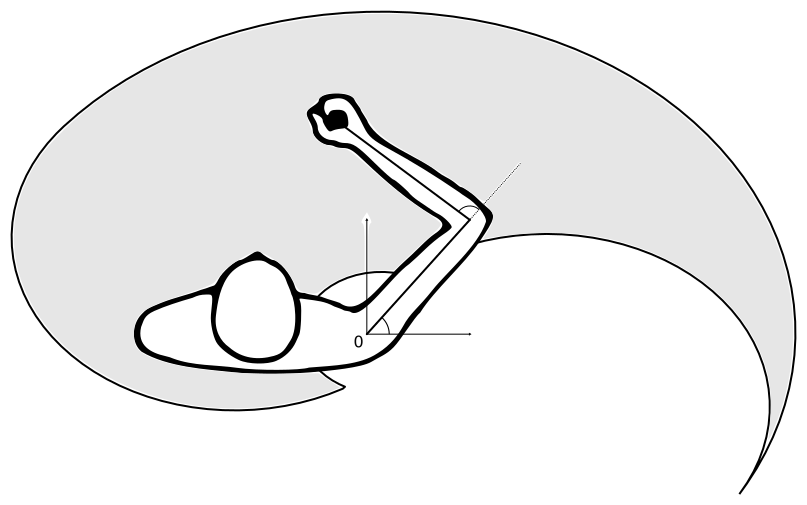
\includegraphics[width=.80\linewidth]{fig/space}
    \caption{Espace de la tâche.}
    \label{fig:space}
\end{figure}

Les équations de la dynamique sont décrites dans \cite{li2006} et les
paramètres utilisés figurent dans l'annexe \ref{app:arm}.

%%%%%%%%%%%%%%%%%%%

\subsubsection{Modèle de muscle}

\begin{figure}[h]
    \centering
    \includegraphics[width=.80\linewidth]{fig/muscles_fr}
    \caption{Vue schématique de l'actionnement musculaire (chaque nombre
    représente un muscle dont le nom est donné en légende).}
    \label{fig:muscles}
\end{figure}

Nous utilisons un modèle de muscle simplifié \cite{rigoux11} pour assurer
l'activation du système. La dynamique des muscles des définie par (\ref{eq:fmax}).
Six muscles (Fig.~\ref{fig:muscles}) permettent de contrôler l'état
$\jstate$ du bras.  Chaque muscle est actionné par un signal d'activation $u_i$
dont la valeur est définie dans l'intervalle $[0 ; 1]$.  Ces signaux produisent
une tension (une force) qui est convertie en couples par la matrice des bras de
leviers. Le contrôle $\jctrl \in \R^6$ est défini
dans l'espace d'action $\mstate$.
Les paramètres utilisés figurent dans l'annexe \ref{app:muscle}.

%%%%%%%%%%%%%%%%%%%

\subsubsection{Paramètres de l'environnement de simulation}

Le simulateur intègre la dynamique du système en utilisant la méthode des
différences finies (méthode d'Euler). Le temps est discrétisé avec un pas
$\Delta_t = 2ms$.
Le critère d'arrêt de la simulation varie suivant les besoins des expériences.

Certaines expériences se déroulent dans un environnement bruité (Fig.~\ref{fig:env-loop}).
Un bruit multiplicatif est alors appliqué sur le contrôle tandis qu'un
bruit additif et un délai perturbent le retour sensoriel.
Pour ces expériences, un estimateur
d'état est adjoint au contrôleur~: il s'agit d'un filtre de Kalman étendu
\cite{kalman1960new}.

\begin{figure}[ht]
    \centering
    \begin{tikzpicture}[scale=1, auto, >=stealth']
    \small

    % TikZ styles for drawing %%%%%%%%%%%%%%%%%%%%%%%%%%%%%%%%%%%%%%%%%%%%%%%%%%%%%%
    \tikzstyle{block} = [draw,rectangle,thick,minimum height=2em,minimum width=2em]
    \tikzstyle{rounded} = [draw,rectangle,rounded corners=2mm,thick,minimum height=2em,minimum width=2em]
    \tikzstyle{sum} = [draw,circle,inner sep=0mm,minimum size=2mm]
    \tikzstyle{connector} = [->,thick]
    \tikzstyle{line} = [thick]
    \tikzstyle{branch} = [circle,inner sep=0pt,minimum size=1mm,fill=black,draw=black]

    % Node placement with matrix library (3x5 array) %%%%%%%%%%%%%%%%%%%%%%%%%%%%%%%%%%%%
    \matrix[ampersand replacement=\&, row sep=0.2cm, column sep=0.5cm] {

      % row 1
      \node[branch, yshift=-2mm] (b2) {}; \&
      \node[block] (control) {Contrôleur}; \&
      \node[rounded] (noise) {Bruit}; \&
      \node[branch] (b3) {}; \&
      \node[block] (model) {Système mécanique (bras)};
      \\

      % row 2
      \&
      \node[sum] (kalman) {K}; \&
      \&
      \&
      \\

      % row 3
      \&
      \&
      \node[rounded] (delta) {Délai}; \&
      \&
      \node[branch] (b4) {};
      \\
    };

     % Now link the nodes %%%%%%%%%%%%%%%%%%%%%%%%%%%%%%%%%%%%%%%%%%%%%%%%%%%%%%%%%%%%%%%%
     \draw [line]      ($(control.west) + (-1cm, 2mm)$) -- ($(control.west) + (-1cm, 2mm)$) node[left] {$\jstate^*$};
     \draw [line]      (b2) -- ($(control.west) + (-1cm, -2mm)$) node[left] {$\jstate_0$};
     \draw [connector] ($(control.west) + (-1cm, 2mm)$) -- ($(control.west) + (0, 2mm)$);
     \draw [connector] (b2) -- ($(control.west) + (0, -2mm)$);
     \draw [connector] (control) -- node {$\jctrl$} (noise);
     \draw [line]      (noise) -- node {$\tilde{\jctrl}$} (b3);
     \draw [connector] (b3) -- (model);
     \draw [connector] (b3) |- (kalman);
     \draw [line]      (model) -- node {$\jstate_{t+1}$} (b4);
%     \draw [connector] (b4) -- ++(2.5cm,0) -- ++(0,3cm) -- ++(-2.5cm,0) -- node {$\jstate_t$} (model.north);
     \draw [connector] (b4) -- (delta);
     \draw [connector] (delta) -| (kalman);
     \draw [line]      (kalman) -| node[pos=0.20] {$\tilde{\jstate}$} (b2);

\end{tikzpicture}

    \caption{Schéma bloc d'une simulation bruitée.}
    \label{fig:env-loop}
\end{figure}

%%%%%%%%%%%%%%%%%%%

%\subsubsection{Paramètres du planifieur QOPS}
%
%Présenter les 3 paramètres et ce qu'ils signifient
%$\costfactor$
%$\rewardfactor$
%$\discountfactor$
%
%Les valeurs que prennent ces trois paramètres sont propres à chaque expérience.
%
%% lamda

%%%%%%%%%%%%%%%%%%%

%\subsubsection{Paramètres du solveur LQP}
%
%?

%%%%%%%%%%%%%%%%%%%%%%%%%%%%%%%%%%%%%%%

\subsection{Conditions expérimentales}

Le module QOPS est codé en C++ avec la bibliothèque
Eigen2 \cite{eigen}.
Au cours de chaque simulation, diverses informations tels que les états
successifs du bras et les commandes d'activations qu'il reçoit sont
enregistrées dans un fichier texte au format CSV.
Ces fichiers sont exploités par des scripts Python/Matplotlib pour générer
les résultats présentés dans ce document.

L'optimisation de la commande dans l'espace des muscles par le LQP est réalisée à l'aide
de la bibliothèque quadprog++ \cite{quadprog}.

Les expériences ont été exécutées sur un processeur AMD Phenom~II~965 avec
2Go de RAM.  Le système d'exploitation utilisé est une distribution Gnu/Linux
Ubuntu~11.04 (AMD64).
Une méthode de planification écrite en Bash a été mise au point afin de
paralléliser les calculs \og{}lourds\fg{} sur plusieurs cœurs de processeur
et/ou plusieurs machines.

%%%%%%%%%%%%%%%%%%%%%%%%%%%%%%%%%%%%%%%

\subsection{Méthodes expérimentales}

Plusieurs expériences sont menées afin d'évaluer la qualité du
contrôleur qui combine QOPS et LQP, que nous nommons QOPS+LQP
dans la suite.

%%%%%%%%%%%%%%%%%%%

\subsubsection{Performance du contrôleur}

Le but de QOPS+LQP est d'offrir une alternative plus légère (en
terme de calcul) au contrôleur présenté dans \cite{rigoux11}.
Il doit donc optimiser les mouvements plus rapidement que ce dernier.
Pour qu'il soit réellement utile, il faut
aussi qu'il génère des solutions d'une qualité proche de ce dernier. Notre
première expérience consiste donc à évaluer la vitesse et la qualité de
ce contrôleur.

Pour ce faire, nous soumettons une tâche identique aux deux
contrôleurs et nous relevons le temps d'exécution de chacun, ainsi que
le coût de la solution générée.

Ce coût est évalué à l'aide de la fonction (\ref{eq:simple-cost-func}).
\begin{equation}
    \label{eq:simple-cost-func}
    \costfuntionhat\left(\jctrl_{\{0..t_f\}}\right) = \sum \jctrl_t^2
\end{equation}

Dans cette expérience, la simulation n'est pas bruitée (le bruit moteur
$\vmotornoise$ et le bruit perceptif $\vperceptionnoise$ sont nuls).
Nous effectuons un mouvement de 10cm d'amplitude, partant
d'une position initiale $\q{}_0 = \begin{pmatrix} 1,0 & 2,0 \end{pmatrix}^T$ radians
(soit $\x{}_0 = \begin{pmatrix} -0,18 & 0,3 \end{pmatrix}^T$ mètres) et allant dans une direction de $90\textdegree$ par rapport à l'axe
des abscisses dans l'espace de la tâche.
Les paramètres du contrôleur sont réglés de façon à obtenir un temps de
mouvement de 450ms.
La simulation est arrêtée dès lors que la vitesse du poignet est inférieure à
5cm/s dans l'espace de la tâche.

%%%%%%%%%%%%%%%%%%%

% TODO : trouver un meilleur titre
\subsubsection{Les invariants du mouvement de haut niveau (dynamique du bras)}

Pour être intéressant, notre contrôleur doit être performant. Mais il doit
aussi vérifier les propriétés connues du contrôle moteur.
Nous pouvons distinguer deux types de propriétés, suivant le niveau
conceptuel qu'elles impactent~: certaines concernant la dynamique du bras
tandis que d'autres sont liées à la variabilité du mouvement.

Nous vérifions tout d'abord que le contrôleur respecte bien les principales
propriétés connues imputables à la dynamique du bras.
Deux expériences seront réalisées dans ce but.

Dans ces deux expériences, 
la simulation n'est pas bruitée (le bruit moteur $\vmotornoise$ et le bruit perceptif
$\vperceptionnoise$ sont nuls) car le bruit ne joue aucun rôle dans les propriétés
mécaniques qu'on essaie de retrouver ici.
Le délai de perception est nul pour les mêmes raisons.
De plus,
les paramètres du contrôleur sont réglés de façon à obtenir un temps de
mouvement proche de celui observé sur des sujets humains dans les mêmes
conditions.
Nous avons ainsi réglé le poids de la récompense $\rewardfactor$ à $4,58.10^5$, le
poids du coût énergétique $\costfactor$ à $3,0.10^3$ et le facteur d'actualisation
$\discountfactor$ à $2,0$.

On considère que chaque mouvement est achevé (cible atteinte) dès que le
poignet a parcouru au moins la moitié de la distance séparant le point de
départ de la cible et que sa vitesse est inférieure à 5cm/s dans
l'espace de la tâche.

%%%

\paragraph{Relation amplitude/durée du mouvement}

% QUOI
\cite{gordon94} a mis en évi\-dence l'existence d'une relation linéaire entre
la durée du mouvement et son amplitude~:
plus l'objectif est éloigné de la position initiale, plus il faut de temps pour
l'atteindre.

Nous souhaitons nous assurer que cette relation est bien conservée par notre
modèle.
% COMMENT
Pour cela, nous lui demandons d'effectuer plusieurs mouvements,
d'amplitude croissante, dont nous mesurons le temps de réalisation.
Le bras part d'une position initiale fixe pour chaque mouvement $\q{}_0 =
\begin{pmatrix} 1,45 & 1,97 \end{pmatrix}^T$ radians (soit environ 
$\begin{pmatrix} -0,3 & 0,2 \end{pmatrix}^T$ mètres). Les cibles sont toutes
réparties sur une même droite, inclinée de $45\textdegree$ par rapport à l'axe
des abscisses dans l'espace de la tâche (Fig.~\ref{fig:scaling-paths}).
Les mouvements sont réalisés pour des amplitudes allant de 10cm à 25cm par pas de 3cm.

\paragraph{Anisotropie}

\cite{gordon94} a également mis en évidence l'existence d'une relation
particulière entre la durée du mouvement et sa direction~:
un mouvement peut être sensiblement plus difficile à exécuter selon la
direction dans laquelle il s'opère.
Cette relation décrit une ellipse dans le système de coordonnées polaires~:
la durée est maximale pour des angles de 0\textdegree et 180\textdegree
et minimale pour des angles de 90\textdegree et 270\textdegree.
%(inverse de la matrice de mobilité).

Nous souhaitons nous assurer que cette relation est bien conservée par notre
modèle.
% COMMENT
Pour cela, nous lui demandons d'effectuer plusieurs mouvements, dans
différentes directions, dont nous mesurons le temps de réalisation.
Le bras part toujours de la position initiale $\q{}_0 = \begin{pmatrix} 1,45 &
1,97 \end{pmatrix}^T$. L'amplitude est fixée à 10cm.
Les mouvements sont réalisés dans des directions allant de 0\textdegree à
360\textdegree par pas de 23\textdegree (0,4 rad). Les cibles sont ainsi réparties
régulièrement, tout au long d'un cercle centré sur le point initial dans
l'espace de la tâche (Fig.~\ref{fig:anisotropy-paths}).

%%%%%%%%%%%%%%%%%%%

\subsubsection{Les invariants du mouvement de bas niveau (muscles)}

%Le \emph{principe de minimisation de la variance} est la principale propriété
%du contrôle moteur connue au niveau musculaire \todo[ref. ?].
%Est-ce que notre modèle respecte cette propriété ?
Les propriétés de variabilité du mouvement humain (principalement la {\em
minimisation de la variance au point final} \cite{harris98_N} et le {\em
principe d'intervention minimum} \cite{todorov02_NN,todorov03_NIPS})
sont en grande partie expliquées
par le fait que le contrôle moteur minimise la variance du mouvement.

Le bloc de bas niveau (LQP) de notre contrôleur effectue une minimisation
(contrainte) des activations musculaires $\jctrl$.  Le bruit moteur $\vmotornoise$ est
proportionnel à $\jctrl$ (bruit multiplicatif), donc en minimisant les activations
musculaires $\jctrl$, on minimise $\vmotornoise$ et par conséquent la
variance du mouvement.

Cette variance est ainsi minimisée localement par le bloc de bas
niveau (LQP). Il nous reste toutefois à montrer que ce principe est respecté
par l'ensemble du contrôleur. On peut imaginer qu'à un niveau global, notre
contrôleur minimise bien la variance, mais il faut s'en convaincre empiriquement.

La \emph{loi de Fitts} et l'allure du \emph{profil de variance au cours
du temps} sont connus pour être des phénomènes émergents du principe de
minimisation de la variance.
Une façon simple de tester notre contrôleur consiste à vérifier que les
mouvements qu'il génère respectent bien la loi de Fitts et la structure de la
variabilité au cours du temps.

Nous mettons en place deux expériences pour cela.
Cette fois, il est nécessaire de prendre en compte les bruits et les délais
dans le contrôle moteur.
Donc un bruit moteur multiplicatif $\vmotornoise$ avec $p(\motornoise) \sim \mathcal{N}(0, 0.4)$ ainsi
qu'un bruit sensoriel additif $\vperceptionnoise$ avec $p(\perceptionnoise) \sim \mathcal{N}(0, 0.0004)$
sont appliqués au cours des simulations. Le délai de perception est fixé à 100ms.

%%%%%%%%

\paragraph{Loi de Fitts}
% QU'EST-CE QUE LA LOI DE FITTS
La loi de Fitts \cite{fitts54_JEP} est un modèle du contrôle moteur humain, prédisant
le temps requis pour aller rapidement d'une position de départ à une cible, en
fonction de la difficulté de la tâche, c'est-à-dire de la distance à parcourir
et de la taille de la cible. Cette loi est définie par l'équation suivante~:

\begin{equation}
    \text{MT} = a + b . \underbrace{\log_2\left(\frac{A}{W}\right)}_\text{ID}
\end{equation}
%\[
%\text{MT} = a + b . \underbrace{\log_2\left(\frac{2A}{W}\right)}_\text{ID}
%\]

Elle établit l'existence d'une relation linéaire entre le temps de réalisation
du mouvement ($\text{MT}$) et une grandeur appelée \emph{l'indice de
difficulté} ($\text{ID}$).
% QU'EST-CE QUE L'INDICE ID ?
Comme son nom l'indique, cet indice exprime la complexité du mouvement réalisé.
Sa valeur dépend de deux paramètres~: la distance séparant la cible de la
position initiale (amplitude $A$ du mouvement) et la taille de la cible ($W$).
La valeur de l'indice de difficulté $\text{ID}$ augmente lorsque l'amplitude du mouvement
augmente et lorsque la taille de la cible diminue.

% QU'EST-CE QU'ON VEUT FAIRE (BUT DE L'EXPÉRIENCE)
Afin de vérifier la loi de Fitts sur notre contrôleur, nous devons mesurer le
temps de réalisation du mouvement ($\text{MT}$) pour différentes valeurs
d'$\text{ID}$, c'est-à-dire pour différentes valeurs d'amplitude $A$ et pour
différentes tailles de cible $W$.
Le paramètre $W$ exprime la variabilité de la position du poignet à la fin du
mouvement (pondérée par un indice de confiance).
Cette variabilité terminale dépend du bruit de l'environnement ($\vmotornoise$ et
$\vperceptionnoise$) mais aussi du facteur de récompense ($\rewardfactor$) et du facteur
d'actualisation ($\discountfactor$) du contrôleur.
En effet, augmenter $\rewardfactor$ ou diminuer $\discountfactor$ revient à
motiver d'avantage le contrôleur et donc la vitesse à laquelle il se dirige sur
la cible. Il en résulte une perte de précision à l'arrivée.
C'est donc par le biais de ces paramètres que nous pouvons modifier la valeur
de W.

Nous avons vu que l'indice de difficulté dépend de plusieurs paramètres.
Nous souhaitons vérifier si la loi de Fitts est globalement respectée par notre
contrôleur, quelle que soit la combinaison de valeurs qu'ils prennent.
Nous mettons donc en place un {\em plan d'expérience factorisé}.
Le bruit est une constante de l'environnement qu'il n'est pas nécessaire
d'inclure dans ce plan.
Il nous reste ainsi trois paramètres à croiser~: l'amplitude $A$ du mouvement,
le facteur de récompense ($\rewardfactor$) et le facteur d'actualisation
($\discountfactor$). Le tableau~\ref{tab:fitts-params} donne l'ensemble de
valeurs retenues pour chacun. Ces valeurs sont choisies de sorte que la durée
du mouvement reste dans l'intervalle [200ms ; 700ms] (délais généralement
appliqués pour des expériences de ce type).
Un ensemble de 27 combinaisons de valeurs est ainsi testé.
Le contrôleur génère 50 mouvements (essais) pour chacune afin d'avoir
suffisamment de positions terminales pour calculer la largeur de la cible
($W$) correspondant à la variance observée.

\begin{table}[htp]
    \centering
    \begin{tabular}{|l|c|c|c|}
        \hline
        amplitude ($A$)                             & 10cm       & 15cm        & 20cm \\
        \hline
        facteur de récompense ($\rewardfactor$)     & $1,4.10^5$ & $4,58.10^5$ & $1,5.10^6$ \\
        \hline
        facteur d'actualisation ($\discountfactor$) & $0,5$      & $1,0$       & $2,0$ \\
        \hline
    \end{tabular}
    \caption{Plan d'expérience}
    \label{tab:fitts-params}
\end{table}

Le bras part d'une position initiale fixe pour chaque mouvement $\q{}_0 =
\begin{pmatrix} 1,8 & 1,9 \end{pmatrix}^T$ radians (soit environ 
$\begin{pmatrix} -0,36 & 0,1 \end{pmatrix}^T$ mètres). Les cibles sont toutes
réparties sur une même droite, inclinée de $45\textdegree$ par rapport à l'axe
des abscisses dans l'espace de la tâche (Fig.~\ref{fig:fitts-paths}).
Comme pour les expériences précédentes, on considère que chaque mouvement est
achevé dès lors que le poignet a parcouru au moins la moitié de la distance
séparant le point de départ de la cible et que sa vitesse est
inférieure à 5cm/s.
Le facteur de coût énergétique est constant $\costfactor=3,0.10^3$. 

%%%%%%%%

\paragraph{Variabilité de la position au cours du temps}

% QUOI
La variabilité de la position du poignet au cours du mouvement décrit un profil
particulier de courbe en cloche tronquée \cite{selen2006impedance}~:
ce qui compte, c'est d'être précis à la fin du mouvement et non pas au milieu.
Cette propriété importante du contrôle moteur a été mise en évidence par
\cite{harris98_N}.

Nous vérifions si notre contrôleur reproduit le même profil.
Pour cela, nous lui demandons d'effectuer une tâche 50 fois dans un environnement bruité.
La variance de la position du poignet est mesurée à chaque pas de temps afin
de tracer un profil dont nous analysons la structure.

Pour chaque mouvement, le bras part d'une position $\q{}_0 =
\begin{pmatrix} 1,8 & 1,9 \end{pmatrix}^T$ radians et se dirige vers une cible
placée à 15cm, dans un angle de 45\textdegree (Fig.~\ref{fig:variability-paths}).
Pour cette expérience, les mouvements ont une durée fixe de 800ms.

Les paramètres du contrôleur ont été réglés pour obtenir un temps de
mouvement proche de celui observé sur des sujets humains dans les mêmes
conditions.
Nous avons ainsi réglé le poids de la récompense $\rewardfactor$ à $1,4.10^5$,
le poids du coût énergétique $\costfactor$ à $3,0.10^3$ et le facteur
d'actualisation $\discountfactor$ à $2,0$.

%%%%%%%%%%%%%%%%%%%%%%%%%%%%%%%%%%%%%%%%%%%%%%%%%%%%%%%%%%%%%%%%%%%%%%%%%%%%%%%

\section{Résultats}
\label{sec:results}

Dans cette partie, nous présentons les résultats obtenus. Nous examinons tout
d'abord les performances du contrôleur. Par la suite, nous mettons en évidence
sa capacité à respecter les principes connus du contrôle moteur.

%%%%%%%%%%%%%%%%%%%

% TODO : on l'appelle comment ce contrôleur ?
\subsection{Performance du contrôleur}

%Les coûts mesurés sont répertoriés dans le tableau \ref{tab:cost-res}. 
%\begin{table}[htp]
%    \centering
%    \begin{tabular}{|l|c|c|c|}
%        \hline
%        Amplitude          & 10cm            & 15cm            & 20cm            \\
%        \hline
%        Durée du mouvement & 330ms           & 400ms           & 460ms           \\
%%        \hline
%%        QOPS               & $1,465.10^{-4}$ & $1,951.10^{-4}$ & $2,121.10^{-4}$ \\
%%        \hline
%%        QOPS+LQP           & $2,015.10^{-4}$ & $3,214.10^{-4}$ & $4,676.10^{-4}$ \\
%        \hline
%%        Coût relatif       & +40\%           & +95\%           &  +102\%         \\
%        Coût relatif       & +40\%           & +\todo\%           &  +\todo\%         \\
%        \hline
%    \end{tabular}
%    \caption{Coût énergétique du mouvement}
%    \label{tab:cost-res}
%\end{table}

Le coût de la trajectoire générée par QOPS+LQP est 40\% plus élevé qu'avec QOPS
pour un temps d'exécution 3 fois plus faible (56 contre 176 secondes).

Les mesures faites ici ne servent que d'indicateur.
%Elles ne remettent pas en cause l'intérêt de notre solution.
Le bénéfice attendu pour le temps d'exécution sera bien plus significatif
avec des systèmes mé\-ca\-niques complexes possédant un grand nombre de 
degrés de liberté (un robot humanoïde par exemple).
Les calculs les plus coûteux sont imputables aux méthodes variationnelles
utilisées par le processus de haut niveau (QOPS).
Plus la taille du vecteur de contrôle est importante, plus les calculs sont coûteux.
Or avec QOPS+LQP, la taille de ce vecteur reste la même quelle que soit
la complexité du système contrôlé.

Pour ce qui est de la qualité des solutions, une majoration de 40\% reste
raisonnable compte tenu des autres bénéfices obtenus, d'autant que rien
n'indique que les sujets humains n'effectuent pas eux aussi un contrôle sous
optimal.
Il est normal que notre contrôleur génère des solutions de qualité moindre car les
activations musculaires sont optimisées avec une fonction de coût
$\costfuntionhat$ (\ref{eq:simple-cost-func}) qui n'est qu'une approximation du
coût $\costfuntion$ (\ref{eq:cost-function}) utilisé pour calculer les
trajectoires dans l'espace de la tâche. Ces trajectoires sont optimales
pour $\costfuntion$ mais par pour $\costfuntionhat$.

%%%%%%%%%%%%%%%%%%%

% TODO : trouver un meilleur titre
\subsection{Respect des invariants du mouvement}

\begin{figure}[p]
    \begin{changemargin}{-3.5cm}{-3.5cm}
      \centering
      \subfloat[Trajectoires]{\label{fig:scaling-paths}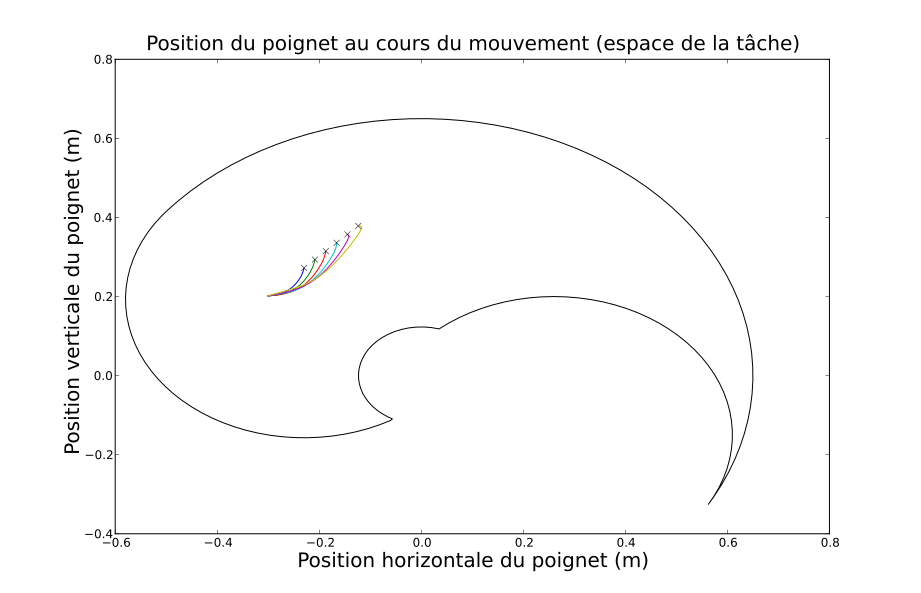
\includegraphics[width=.50\linewidth]{fig/lqp_scaling_paths}}
      \subfloat[Résultat]{\label{fig:scaling-res}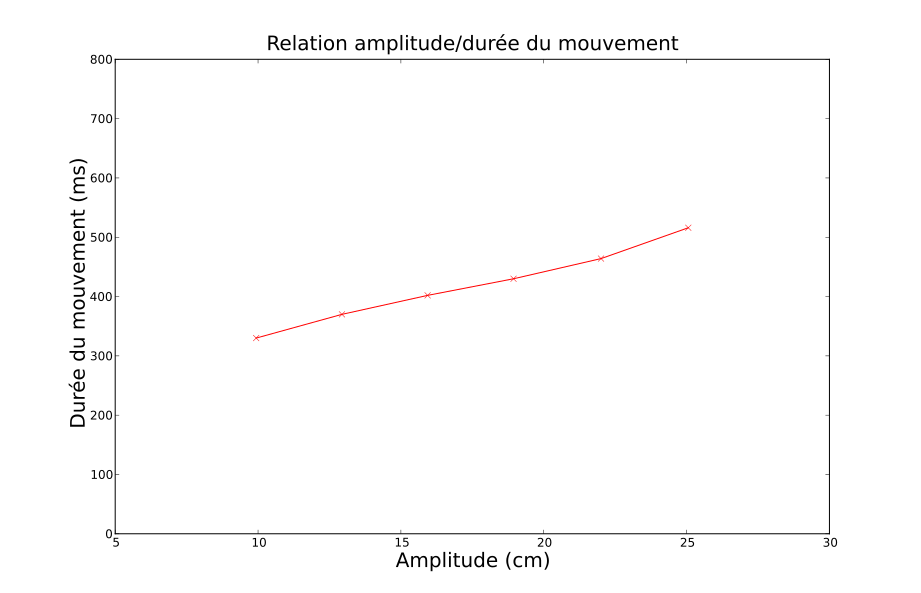
\includegraphics[width=.50\linewidth]{fig/lqp_scaling}}
      \caption{Relation amplitude/durée du mouvement}
      \label{fig:scaling}
    \end{changemargin}
\end{figure}

\begin{figure}[p]
    \begin{changemargin}{-3.5cm}{-3.5cm}
      \centering
      \subfloat[Trajectoires]{\label{fig:anisotropy-paths}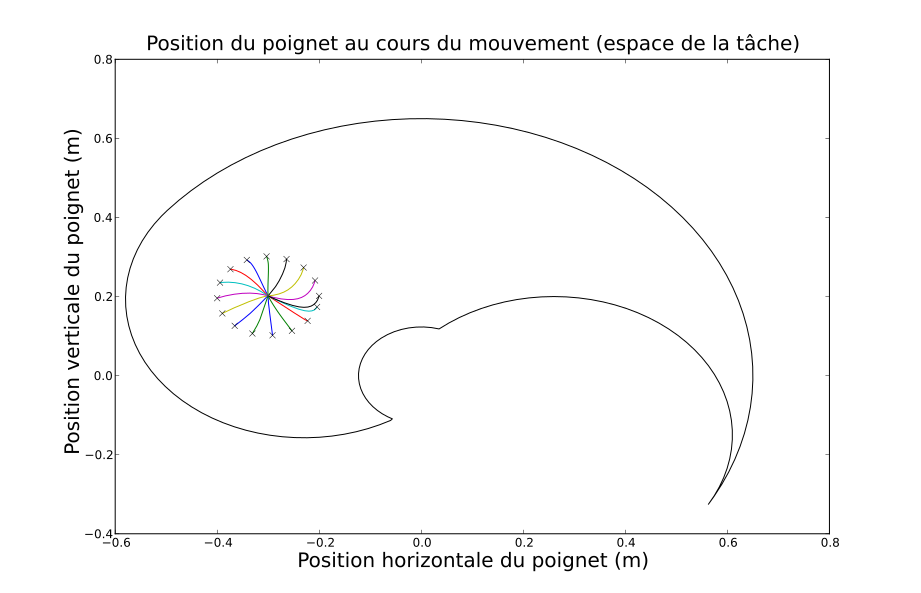
\includegraphics[width=.50\linewidth]{fig/lqp_anisotropie_paths}}
      \subfloat[Résultat]{\label{fig:anisotropy-res}\includegraphics[width=.50\linewidth]{fig/lqp_anisotropie}}
      \caption{Anisotropie}
      \label{fig:anisotropy}
    \end{changemargin}
\end{figure}

% TODO : trouver un meilleur titre
\subsubsection{Relation amplitude/durée du mouvement}

Nous pouvons constater sur la figure \ref{fig:scaling-res} que le temps de
réalisation des mouvements générés par notre contrôleur est d'autant plus long que la
cible est plus éloignée de la position initiale du poignet
(Fig.~\ref{fig:scaling-paths}).
Nous pouvons également remarquer que cette relation durée/amplitude est linéaire.
La relation de \cite{gordon94} est bien conservée par notre modèle.

\subsubsection{Anisotropie}

Nous pouvons constater sur la figure \ref{fig:anisotropy-res} qu'il existe une
corrélation entre la durée du mouvement généré par notre contrôleur et sa direction
(Fig.\ref{fig:anisotropy-paths}). 
%La relation qui lie la durée du mouvement et sa direction décrit des variations
Nous pouvons également remarquer que la relation représentée sur la figure
\ref{fig:anisotropy-res} décrit des variations similaires à celle mise en
évidence par \cite{gordon94}.
%(l'inverse de la matrice de mobilité).
La durée du mouvement est maximale pour des angles de 0\textdegree et 180\textdegree
et minimale pour des angles de 90\textdegree et 270\textdegree.
Notre contrôleur conserve bien la relation d'anisotropie.

\subsubsection{Loi de Fitts}

\begin{figure}[p]
    \begin{changemargin}{-3.5cm}{-3.5cm}
      \centering
      \subfloat[Trajectoires]{\label{fig:fitts-paths}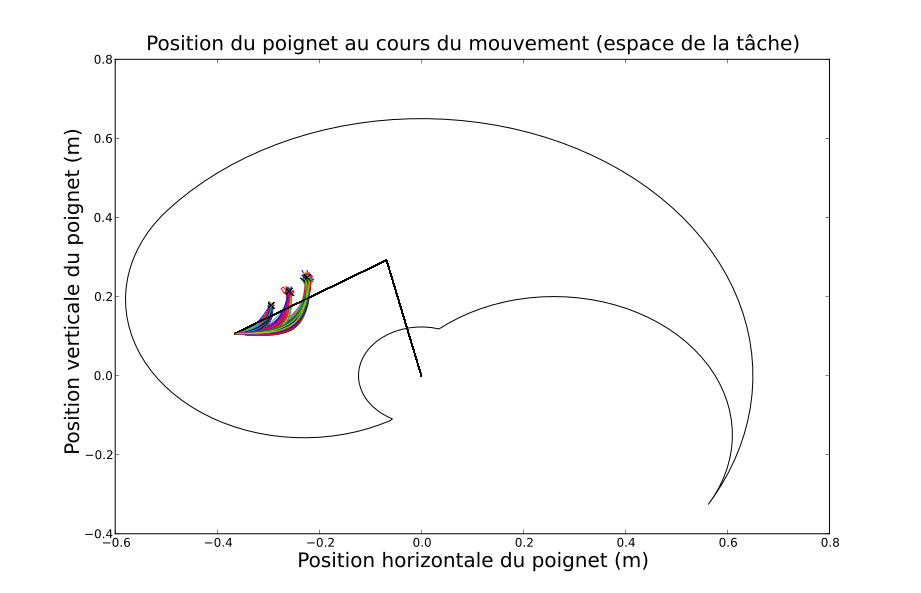
\includegraphics[width=.50\linewidth]{fig/lqp_fitts_paths}}
      \subfloat[Résultat]{\label{fig:fitts-res}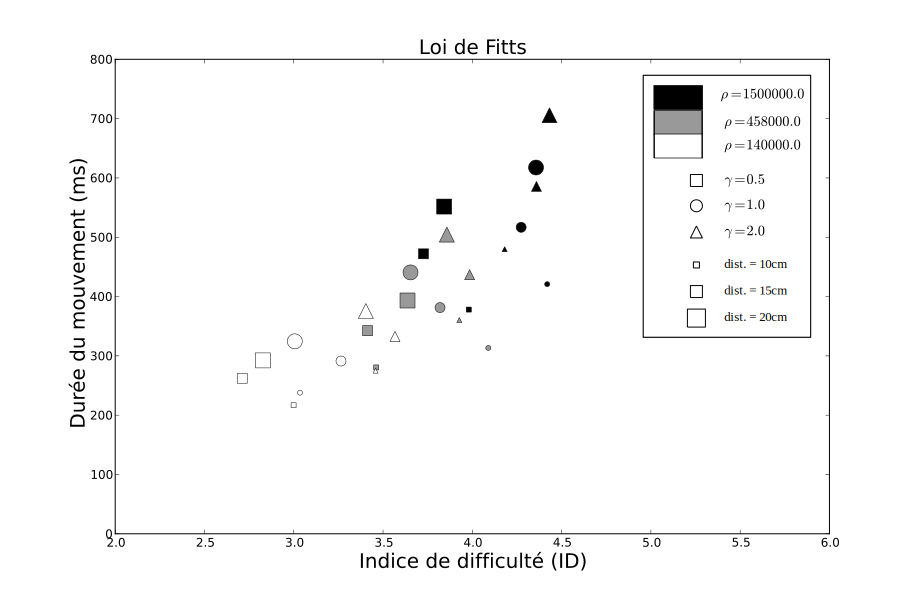
\includegraphics[width=.50\linewidth]{fig/lqp_fitts2_sigma4}}
      \caption{Loi de Fitts}
      \label{fig:fitts}
    \end{changemargin}
\end{figure}

\begin{figure}[p]
    \begin{changemargin}{-3.5cm}{-3.5cm}
      \centering
      \subfloat[Trajectoires]{\label{fig:variability-paths}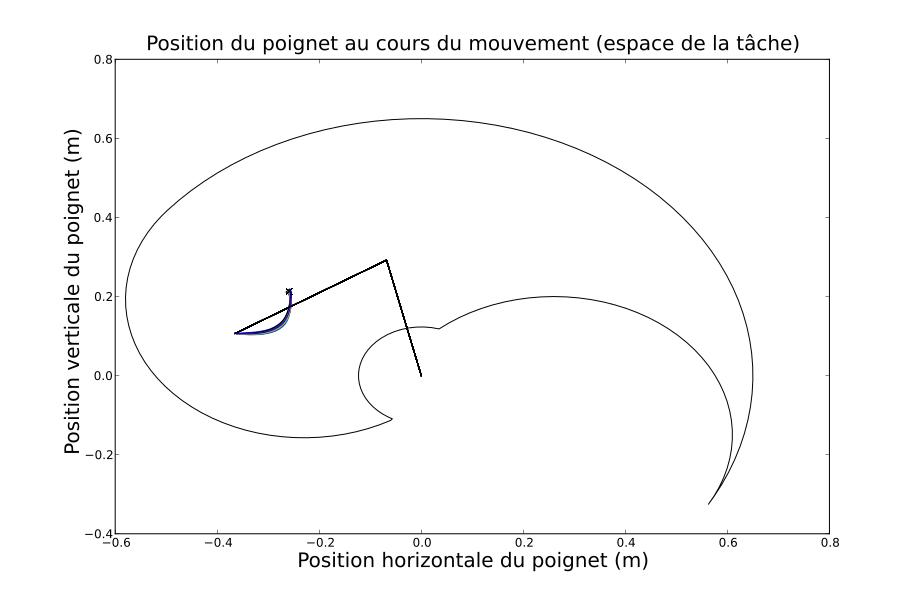
\includegraphics[width=.50\linewidth]{fig/lqp_variations_paths}}
      \subfloat[Résultat]{\label{fig:variability-res}\includegraphics[width=.50\linewidth]{fig/lqp_variation_exp5}}
      \caption{Variabilité de la position au cours du temps}
      \label{fig:variability}
    \end{changemargin}
\end{figure}

La figure \ref{fig:fitts-res} montre la durée moyenne du mouvement mesurée pour
différents indices de difficulté.
Nous pouvons voir 27 points correspondant aux 27 combinaisons de valeurs
testées pour les trois paramètres dont dépend la valeur ID ($\discountfactor$,
$\rewardfactor$ et $A$).  Pour chaque point, le contrôleur a généré 50
mouvements à partir desquels nous calculons la variabilité de la position
terminale $\sigma$ et le temps moyen de réalisation du mouvement $MT$.
La valeur de $\sigma$ est pondérée par un indice de confiance (3,92 pour
retenir 95\% de la population) afin de calculer la largeur de la cible $W$
et la valeur ID correspondant à ce point.
%$\text{ID} = \log_2\left(\frac{A}{W}\right)$ avec $W = 3,92 . \sigma$.

%Nous pouvons remarquer sur la figure\ref{fig:fitts-res} que les mouvements générés
Nous pouvons remarquer que les mouvements générés par notre modèle sont d'autant
plus longs que leur indice de difficulté (ID) est élevé.
Nous pouvons également remarquer que la relation qui lie ces deux quantités est
linéaire, ce qui est conforme à la loi de Fitts. 
%Notre contrôleur vérifie la loi de Fitts.

%\ref{fig:fitts-paths}

% TODO : trouver un meilleur titre
\subsubsection{Variabilité de la position au cours du temps}

La figure \ref{fig:variability-res} montre la variabilité de la position du
poignet au cours des 50 mouvements générés par notre contrôleur.  La cible est
atteinte\footnote{d'après les critères utilisés dans les autres expériences} au
bout de 600ms en moyenne.  Nous pouvons remarquer que la variance est maximale
en milieu de mouvement conformément au principe du minimum d'intervention.
Nous pouvons également noter que la variance est minimale à la fin du
mouvement, conformément au principe de minimisation de la variance au point
final.

%Le profil mesurée est similaire aux résultats empiriques .
Notre contrôleur reproduit le profil particulier mesuré par \cite{selen2006impedance}.
Cette propriété est donc bien conservée.

%%%%%%%%%%%%%%%%%%%%%%%%%%%%%%%%%%%%%%%%%%%%%%%%%%%%%%%%%%%%%%%%%%%%%%%%%%%%%%%

\section{Discussion}
\label{sec:discu}

%%%%%%%%%%%%%%%%%%%%%%%%%%%%%%%%%%%%%%%

%\subsection{La trajectoire désirée}
\paragraph{}

Pour \cite{todorov02_NN}, une séparation stricte entre le processus de planification de la
trajectoire et son exécution ne permet pas de reproduire les propriétés
connues du contrôle moteur.
Ces propriétés sont pourtant vérifiées par notre contrôleur qui peut être vu
comme le découplage de deux processus~:
l'un chargé de planifier une trajectoire dans l'espace opérationnel et l'autre
chargé de l'exécuter au niveau musculaire.
Notre modèle échappe aux critiques de \cite{todorov02_NN} pour plusieurs raisons.

Tout d'abord, dans le cas d'un système redondant, la trajectoire calculée dans l'espace
opérationnel peut être spécifiée sans pour autant qu'elle soit définie par une unique trajectoire
dans l'espace articulaire. En fait, c'est essentiellement lors du passage de
l'espace opérationnel à l'espace articulaire que le principe d'intervention
minimum entre en jeu \cite{todorov02_NN,todorov03_NIPS}.

De plus, les arguments avancés par \cite{todorov02_NN} à l'encontre d'une \og{}trajectoire désirée\fg{}
ne s'appliquent qu'à des modèles fonctionnant en boucle ouverte, c'est-à-dire
où la trajectoire est d'abord planifiée puis entièrement exécutée, sans retour sensoriel.
Or, dans notre cas, le contrôleur fonctionne en boucle fermée~: il perçoit une approximation
de l'état réel du système à chaque pas de temps et il s'en sert pour mettre à jour 
la trajectoire \cite{guigon08b}.

Enfin, le processus d'optimisation de haut niveau génère la \og{}trajectoire
désirée\fg{} dans l'espace de la tâche et non pas dans l'espace articulaire.
La méthode de contrôle optimal qui exécute la trajectoire %dans l'espace musculaire
résout les redondances articulaires et musculaires et reproduit ainsi le principe
d'intervention minimum proposé dans \cite{todorov02_NN,todorov03_NIPS}.

Au final, QOPS+LQP peut être vu comme une idéalisation du modèle proposé par \cite{shadmehr05},
où le but est spécifié dans l'espace de travail (en pratique, l'espace visuel),
une trajectoire désirée est calculée dans ce même espace
et un contrôleur de plus bas niveau actionne les muscles pour l'exécuter
dans l'espace musculaire.

%%%%%%%%%%%%%%%%%%%%%%%%%%%%%%%%%%%%%%%

%\subsection{Peut-on améliorer l'architecture~?}

\paragraph{}
Il existe plusieurs façons de simplifier le problème d'optimisation du con\-trô\-le
moteur. Nous avons choisi d'approcher la fonction de coût utilisée dans
\cite{rigoux11} en utilisant une force $\octrl$ définie dans
l'espace opérationnel plutôt que des activations musculaires $\jctrl$.

Une alternative plus économe en temps de calcul consisterait à approcher la dynamique
du bras par une masse ponctuelle.
L'optimisation de la trajectoire (le processus de haut niveau) serait alors
plus rapide qu'avec notre modèle.
Cette solution devrait suffire à reproduire la relation durée/amplitude
qui ne dépend pas de la géométrie du système mais pas la propriété
d'ani\-so\-tro\-pie qui, elle, en dépend.

Une autre option (Fig.\ref{fig:solutions}c) consisterait à optimiser la trajectoire du bras dans l'espace
articulaire $\jstate$ plutôt que dans l'espace d'actionnement $\mstate$.
On optimiserait alors un vecteur de couples $\vt^*$ dans le processus de haut niveau
puis on chercherait le vecteur d'activations musculaires optimale $\jctrl^*$
permettant de réaliser ce couple.
Cette solution coûte moins chère à l'exécution que celle proposée dans \cite{rigoux11}
mais elle est plus chère que la nôtre car l'optimisation de la trajectoire
est réalisée dans l'espace des articulations $\jstate$ qui reste un espace de
grande taille pour des systèmes mécaniques poly-articulés complexes.
Comme notre modèle reproduit les principales propriétés du contrôle moteur pour
des coûts de mouvements relativement proches de l'optimal, cette complexité
supplémentaire n'est pas nécessaire.
Il faudrait tout de même déterminer si l'impact de cette approche sur le coût
énergétique des meilleurs mouvements trouvés est moindre.

%%%%%%%%%%%%%%%%%%%%%%%%%%%%%%%%%%%%%%%

%%\subsection{Une approche plus intuitive}
%
%\paragraph{}
%Certains arguments nous laissent penser qu'une transformation explicite de
%l'espace de la tâche vers l'espace articulaire est effectuée dans notre
%cerveau.
%La cible du mouvement est généralement acquise par la vision.  L'état de cette
%cible est donc probablement codée dans l'espace visuel.  De même, le retour
%perceptif, essentiellement visuel\todo[pas sûr, la proprioception est sûrement
%plus importante], est probablement codé dans l'espace visuel.
%
%Une vision alternative du problème consisterait à considérer que le
%but est spécifié dans l'espace de la tâche puis transformé en
%un état à atteindre dans l'espace articulaire avant d'être intégré
%dans la fonction de coût \todo[correct?].
%
%En effet, optimiser dans l'espace musculaire n'explique pas pourquoi
%nous avons l'intuition que notre mouvement est dirigé dans une
%certaine direction de l'espace. L'hypothèse proposée ici rend le 
%mécanisme d'optimisation plus naturel et plus intuitif.
%
%\todo

%%%%%%%%%%%%%%%%%%%%%%%%%%%%%%%%%%%%%%%

%%\subsection{Le coût d'exécution}
%\paragraph{}
%
%\todo

%%%%%%%%%%%%%%%%%%%%%%%%%%%%%%%%%%%%%%%

%\subsection{Perspectives}
\paragraph{}

LQP+QOPS présente quelques limitations.  En particulier, nous
n'utilisons qu'un modèle simplifié de muscles linéaires, l'espace de travail de
la tâche est défini de sorte à éviter les butées articulaires, nous ne
considérons pas la présence d'obstacles et nous supposons que la trajectoire
calculée dans l'espace de la tâche peut toujours être exécutée par les muscles,
ce qui n'est pas vrai dans le cas général.

Ces limitations résultent de choix d'implémentation guidés par un souci de
rapidité d'exécution.  Elles ne remettent pas en cause la validité de notre
modèle.  De plus, il serait relativement aisé de tenir compte des contraintes
géométriques à tous les niveaux en remplaçant les outils d'optimisation
utilisés par un outil plus générique tel qu'Ipopt \cite{ipopt}.

Le contrôle opéré au niveau des muscles tente de reproduire réactivement les forces
qui sont immédiatement requises pour suivre la trajectoire optimale dans l'espace de la tâche.
Plutôt qu'une approche réactive, nous pourrions imaginer un contrôleur de
muscles recevant à l'avance les forces à exécuter, en anticipant la trajectoire
calculée dans l'espace opérationnel.
Implémenter cette idée nécessiterait l'utilisation de méthodes de contrôle prédictif.
Bien que cela rende le modèle plus coûteux en calculs, il serait toujours plus rapide
que la solution proposée par \cite{rigoux11}.

Enfin, notre travail ouvre des perspectives pour l'apprentissage du con\-trô\-le moteur.
À cause de la \og{}malédiction de la dimensionalité\fg{}, l'apprentissage de
politiques de contrôle optimales est contraint par
le nombre de dimensions du système. Les méthodes employées aujourd'hui ne permettent
pas d'apprendre sur des systèmes complexes tel qu'un robot humanoïde.
Apprendre un contrôleur optimal dans l'espace de la tâche (sans tenir compte
des articulations ou des muscles) rend le problème beaucoup plus accessible
en terme de coût du calcul.
Grâce à cette approche simplifiée, nous pouvons espérer résoudre la question de l'adaptation motrice et de la
réoptimisation étudiées dans \cite{izawa08} et appliquées dans \cite{marin11_gecco}.
En particulier, notre modèle ouvre des perspectives dans l'apprentissage
de phénomènes du contrôle moteur qui requièrent de la redondance pour être étudiés
tels que \cite{diedrichsen10}.


%%%%%%%%%%%%%%%%%%%%%%%%%%%%%%%%%%%%%%%%%%%%%%%%%%%%%%%%%%%%%%%%%%%%%%%%%%%%%%%%

\newpage

\appendix

%\section{Mécanique du bras}
\section{Paramètres du bras}
\label{app:arm}

%%%%%%%%%%%%%%%%%%%%
%
%\subsubsection{Notations}
%
%\begin{figure}[h]
%    \centering
%    \includegraphics[width=.60\linewidth]{fig/arm2_fr}
%    \caption{Vue schématique de la mécanique du modèle de bras utilisé.}
%    \label{fig:app-arm}
%\end{figure}
%
%\begin{tabular}{ll}
%  $\ms{M}(\q) \in \mathbb{R}^{2 \times 2}$ & Matrice d'inertie \\
%  $\vs{C}(\q, \dq) \in \mathbb{R}^{2}$     & Force de Coriolis et force centrifuge \\
%  $\vs{B}(\dq) \in \mathbb{R}^{2}$         & Force de viscosité et de friction \\
%  $\vt \in \mathbb{R}^{2}$                 & Couple total exercé sur les articulations ($N \cdot m$) \\
%  $\ddq \in \mathbb{R}^{2}$                & Accélération angulaire des articulations ($rd \cdot s^{-2}$) \\
%  $\dq \in \mathbb{R}^{2}$                 & Vitesse angulaire des articulations ($rd \cdot s^{-1}$)\\
%  $\q \in \mathbb{R}^{2}$                  & Angle des articulations ($rd$)\\
%  $\jstate \in \mathbb{R}^{4}$             & État du bras dans l'espace articulaire ($rd$)\\
%  $\ostate \in \mathbb{R}^{4}$             & État du bras dans l'espace de la tâche ($m$)\\
%\end{tabular}
%
%%%%%%%%%%%%%%%%%%%%
%
%\subsubsection{Représentation de l'état}
%
%Dans l'{\em espace articulaire}~:
%\begin{equation}
%    \jstate = \begin{pmatrix} \dq \\ \q \end{pmatrix} = \begin{pmatrix} \dqs \\ \dqe \\ \qs \\ \qe \end{pmatrix}
%\end{equation}
%
%Dans l'{\em espace de la tâche} (ou {\em espace opérationnel})~:
%\begin{equation}
%    \ostate = \begin{pmatrix} \dx \\ \x \end{pmatrix} = \begin{pmatrix} \dxx \\ \dxy \\ \xx \\ \xy \end{pmatrix}
%\end{equation}
%
%%%%%%%%%%%%%%%%%%%%
%
%\subsubsection{Transformations cinématiques}
%
%Cinématique (de l'espace articulaire à l'espace de la tâche)~:
%\begin{align*}
%  \xx & = \lu \cosqs + \lf \cosqsqe \\
%  \xy & = \lu \sinqs + \lf \sinqsqe \\
%\end{align*}
%
%Cinématique inverse (de l'espace de la tâche vers l'espace articulaire)~:
%\begin{align*}
%  r   & = \sqrt{\xx^2 + \xy^2} \\
%  \qs & = \arctan2(\xy, \xx) - \arccos \left( \frac{r^2 + \lu^2 - \lf^2}{2 \lu r} \right) \\
%  \qe & = \arccos \left( \frac{r^2 - \lu^2 - \lf^2}{2 ~ \lu \lf} \right) \\
%\end{align*}
%
%%%%%%%%%%%%%%%%%%%%
%
%\subsubsection{Jacobienne}
%\begin{align*}
%  \jacobian & = \begin{pmatrix}J_{11} & J_{12} \\ J_{21} & J_{22}\end{pmatrix} \\
%         & = \begin{jmatrix}
%               \pd{\xx}{\qs} & \pd{\xx}{\qe} \\
%               \pd{\xy}{\qs} & \pd{\xy}{\qe}
%             \end{jmatrix} \\
%         & = \begin{jmatrix}
%               -\lu \sinqs - \lf \sinqsqe &
%               -\lf \sinqsqe \\
%                \lu \cosqs + \lf \cosqsqe &
%                \lf \cosqsqe
%             \end{jmatrix} \\
%\end{align*}
%
%%%%%%%%%%%%%%%%%%%%
%
%\subsubsection{Transformations dynamiques}
%
%Dynamique (des forces aux accélérations)~:
%\begin{align*}
%    \ddq & = \ms{M}(\q)^{-1} (\vt - \ms{C}(\q, \dq) \dq - \ms{B} \dq - \vs{g}(\q)) 
%\end{align*}
%
%Dynamique inverse (des accélérations aux forces)~:
%\begin{equation}
%    \vt = \ms{M}(\q) \ddq + \ms{C}(\q, \dq) \dq + \ms{B} \dq + \vs{g}(\q)
%\end{equation}
%
%%%%%%%%%%%%%%%%%%%%
%
%\subsubsection{Raccourcis}
%\begin{align*}
%  \scut_1 & = \is + \ie + \mf \lu^2 + \msu \dcmu^2 + \mf \dcmf^2 \\
%  \scut_2 & = \mf \lu \dcmf \\
%  \scut_3 & = \ie + \mf \dcmf^2 \\
%  \scut_4 & = -\mf \lu \dcmf \sinqe 
%\end{align*}
%
%%%%%%%%%%%%%%%%%%%%

%\subsubsection{Paramètres}

\begin{tabular}{ll}
  $\m_i$   & Masse du membre $i$ ($kg$) \\
  $\len_i$ & Longueur du membre $i$ ($m$) \\
  $\dcm_i$ & Distance séparant le centre de l'articulation $i$ au centre de masse du membre $i$ ($m$) \\
  $\si_j$  & Moment d'inertie de l'articulation $j$ sur le centre de mass du membre $j$ ($kg \cdot m^2$) \\
\end{tabular}

\begin{align*}
  \begin{pmatrix} \msu  \\ \mf   \end{pmatrix} & = \begin{pmatrix} 1.4               \\ 1.1  \end{pmatrix} \\
  \begin{pmatrix} \lu   \\ \lf   \end{pmatrix} & = \begin{pmatrix} 0.3               \\ 0.35 \end{pmatrix} \\
  \begin{pmatrix} \dcmu \\ \dcmf \end{pmatrix} & = \begin{pmatrix} 0.11              \\ 0.16 \end{pmatrix} \\
  \begin{pmatrix} \is   \\ \ie   \end{pmatrix} & = \begin{pmatrix} 2.5 \cdot 10^{-2} \\ 4.5  \cdot 10^{-2} \end{pmatrix} 
\end{align*}

%%%%%%%%%%%%%%%%%%%%
%
%\subsubsection{Matrice d'inertie}
%\begin{align*}
%  \ms{M}(\q)      = {} & \begin{pmatrix} M_{11} & M_{12} \\ M_{21} & M_{22} \end{pmatrix} \\
%                  = {} & \begin{pmatrix}
%                           \scut_1 + 2 \scut_2 \cosqe  & \scut_3 + \scut_2 \cosqe \\
%                           \scut_3 + \scut_2 \cosqe    & \scut_3 \\
%                         \end{pmatrix} \\
%  \detM           = {} & M_{22} M_{11} - M_{12} M_{21} \\
%                  = {} & \scut_3 ( \scut_1 + 2 \scut_2 \cosqe) - 2 (\scut_3 + \scut_2 \cosqe) \\
%                  = {} & \ie \is + \ie \msu \dcmu^2 + \ie \mf \lu^2 + \mf \dcmf^2 \is\\
%                       & + \msu \mf \dcmu^2 \dcmf^2 + \mf^2 \dcmf^2 \lu^2 - \mf^2 \lu^2 \dcmf^2 \cos^2(\qe) \\
%  \ms{M}^{-1}(\q) = {} & \begin{pmatrix} \invM{11} & \invM{12} \\ \invM{21} & \invM{22} \end{pmatrix} \\
%                  = {} & \frac{1}{\detM} \begin{pmatrix} M_{22} & -M_{12} \\ -M_{21} & M_{11} \end{pmatrix} \\
%                  = {} & \begin{jmatrix} \frac{M_{22}}{\detM} & \frac{-M_{12}}{\detM} \\ \frac{-M_{21}}{\detM} & \frac{M_{11}}{\detM} \end{jmatrix} \\
%\end{align*}
%
%%%%%%%%%%%%%%%%%%%%
%
%\subsubsection{Autres forces}
%\begin{align*}
%  \vs{C}(\q, \dq) & = \begin{pmatrix} \scut_4 \dqe & \scut_4 (\dqs + \dqe) \\ -\scut_4 \dqs & 0 \end{pmatrix} \\
%  \vs{B}          & = \begin{pmatrix} b_{11} & b_{12} \\ b_{21} & b_{22} \end{pmatrix} \\
%                  & = \begin{pmatrix} 0.05  & 0.025 \\ 0.025 & 0.05 \end{pmatrix} \\
%  \vs{n}(\q, \dq) & = \ms{C}(\q, \dq) \dq + \ms{B} \dq + \vs{g}(\q)  \\
%                  & = \ms{C}(\q, \dq) \dq + \ms{B} \dq \\
%                  & = \begin{pmatrix}n_1 \\ n_2\end{pmatrix} \\
%                  & = \begin{pmatrix}
%                        -2 ~ \mf ~ \lu ~ \dcmf ~ \sinqe ~ \dqe ~ \dqs - \mf ~ \lu ~ \dcmf ~ \sinqe ~ \dqe^2 + b_{11} ~ \dqs + b_{12} ~ \dqe \\
%                        \mf ~ \lu ~ \dcmf ~ \sinqe ~ \dqs^2 + b_{21} ~ \dqs + b_{22} ~ \dqe 
%                      \end{pmatrix} \\
%\end{align*}

%%%%%%%%%%%%%%%%%%%%%%%%%%%%%%%%%%%%%%%

\section{Paramètres des muscles}
%\section{Modèle de muscles}
\label{app:muscle}

%%\subsubsection{Notations}
%\begin{figure}[h]
%    \centering
%    \includegraphics[width=.60\linewidth]{fig/muscles_fr}
%    \caption{Vue schématique de l'actionnement musculaire (chaque nombre
%             représente un muscle dont le nom est donné en légende).}
%    \label{fig:app-muscles}
%\end{figure}
%
%\begin{small}
%  \begin{tabular}{ll}
%    $\vt \in \mathbb{R}^2$                                      & Couple total exercé sur les articulations ($N \cdot m$) \\
%    $\ms{A} \in \mathbb{R}^{6 \times 2}$                        & Matrice des bras de levier ($m$) \\
%    $\jctrl \in \mathbb{R}^6$                                   & Activations musculaires $(u_i \in [0;1])$ \\
%    $\vs{f_{\max}} \in \mathbb{R}^6$                            & Force maximale pouvant être produite par chaque muscle $(N)$ \\
%    $\text{diag}(\vs{f_{\max}}) \cdot \jctrl \in \mathbb{R}^6$  & Tension (force) exercée par chaque muscle $(N)$
%  \end{tabular}
%\end{small}

%%%%%%%%%%%%%%%%%%%

%\subsubsection{Filtres}
%\begin{align*}
%  [u]^+             & = \frac{\log(e^{\kappa u} + 1)}{\kappa}  \\
%  \frac{d[u]^+}{du} & = \frac{e^{\kappa u}}{e^{\kappa u} + 1}  \\
%\end{align*}
%
%\begin{figure}[h]
%    \centering
%    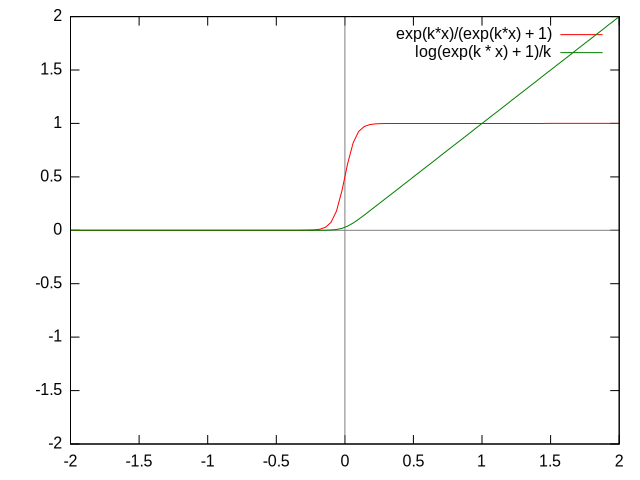
\includegraphics[width=.40\linewidth]{fig/filter}
%    \caption{Fonctions $[u]^+$ et $d[u]^+/du$.}
%    \label{fig:app-filter}
%\end{figure}
%
%%%%%%%%%%%%%%%%%%%%
%
%\subsubsection{Dynamique du muscle}
%\begin{align*}
%  \vs{f_{\max}} & = \begin{pmatrix}f_{\max1} & f_{\max2} & f_{\max3} & f_{\max4} & f_{\max5} & f_{\max6}\end{pmatrix}^T \\
%                & = \begin{pmatrix}700 & 382 & 572 & 445 & 159 & 318\end{pmatrix}^T \\
%                & \\
%  \ms{A}^T      & = \begin{pmatrix}A_{11} & A_{21} & A_{31} & A_{41} & A_{51} & A_{61} \\
%                                   A_{12} & A_{22} & A_{32} & A_{42} & A_{52} & A_{62} \\\end{pmatrix} \\
%                & = \begin{pmatrix}0.04 & -0.04 & 0     & 0      & 0.028 & -0.035 \\
%                                   0    & 0     & 0.025 & -0.025 & 0.028 & -0.035 \\\end{pmatrix} \\
%                & \\
%  \vt           & = \begin{pmatrix}\ts & \te\end{pmatrix}^T \\
%%                & = \ms{A}^T ~ \text{diag}(\vs{f_{\max}}) ~ \vs{[u]^+} \\
%%                & = \begin{pmatrix}
%%                      A_{11} ~ f_{\max1} ~ [u_1]^+ + A_{21} ~ f_{\max2} ~ [u_2]^+ + A_{51} ~ f_{\max5} ~ [u_5]^+ + A_{61} ~ f_{\max6} ~ [u_6]^+ \\
%%                      A_{32} ~ f_{\max3} ~ [u_3]^+ + A_{42} ~ f_{\max4} ~ [u_4]^+ + A_{52} ~ f_{\max5} ~ [u_5]^+ + A_{62} ~ f_{\max6} ~ [u_6]^+ \\
%                & = \ms{A}^T ~ \text{diag}(\vs{f_{\max}}) ~ \jctrl \\
%                & = \begin{pmatrix}
%                      A_{11} ~ f_{\max1} ~ u_1 + A_{21} ~ f_{\max2} ~ u_2 + A_{51} ~ f_{\max5} ~ u_5 + A_{61} ~ f_{\max6} ~ u_6 \\
%                      A_{32} ~ f_{\max3} ~ u_3 + A_{42} ~ f_{\max4} ~ u_4 + A_{52} ~ f_{\max5} ~ u_5 + A_{62} ~ f_{\max6} ~ u_6 \\
%                    \end{pmatrix} \\
%\end{align*}
\begin{align*}
  \vs{f_{\max}} & = \begin{pmatrix}700 & 382 & 572 & 445 & 159 & 318\end{pmatrix}^T \\
  \ms{A}^T      & = \begin{pmatrix}0.04 & -0.04 & 0     & 0      & 0.028 & -0.035 \\
                                   0    & 0     & 0.025 & -0.025 & 0.028 & -0.035 \\\end{pmatrix} \\
\end{align*}
Les valeurs sont tirées de \cite{katayama1993} (pp. 356-357).

%%%%%%%%%%%%%%%%%%%%%%%%%%%%%%%%%%%%%%%%%%%%%%%%%%%%%%%%%%%%%%%%%%%%%%%%%%%%%%%%

\newpage

%\bibliographystyle{plain}
\bibliographystyle{alpha}
\bibliography{article}

\end{document}
